%%%%%%%%%%%%%%%%%%%%%%%%%%%%%%%%%%%%%%%%%%%%%%%%%%%%%%%%%%%%%%%%%%%%%%%%%%%%%%%% 
%
%   Basic configuration
%
%%%%%%%%%%%%%%%%%%%%%%%%%%%%%%%%%%%%%%%%%%%%%%%%%%%%%%%%%%%%%%%%%%%%%%%%%%%%%%%%

% Use 'KOMA-Script Book' as the document class
\documentclass[toc=bibliography,toc=indentunnumbered,listof=totoc]{scrbook}



%%%%%%%%%%%%%%%%%%%%%%%%%%%%%%%%%%%%%%%%%%%%%%%%%%%%%%%%%%%%%%%%%%%%%%%%%%%%%%%%
%
%   Preload essentials
%
%%%%%%%%%%%%%%%%%%%%%%%%%%%%%%%%%%%%%%%%%%%%%%%%%%%%%%%%%%%%%%%%%%%%%%%%%%%%%%%%

% Load some required packages
\usepackage{etoolbox}                   % Modding standard environments
\usepackage[fleqn,intlimits]{amsmath}   % Common mathematical environments
\usepackage[svgnames]{xcolor}           % Enables coloring of text and pages
\usepackage{hyperref}                   % Enables hyperlink generation



%%%%%%%%%%%%%%%%%%%%%%%%%%%%%%%%%%%%%%%%%%%%%%%%%%%%%%%%%%%%%%%%%%%%%%%%%%%%%%%%
%
%   Page design
%
%%%%%%%%%%%%%%%%%%%%%%%%%%%%%%%%%%%%%%%%%%%%%%%%%%%%%%%%%%%%%%%%%%%%%%%%%%%%%%%%

% Font size
\KOMAoptions{fontsize=11pt}

% Line spacing
\linespread{1.07} 

% Paper format
\KOMAoptions{paper=B5}

% Duplex layout
\KOMAoptions{twoside}

% Page layout (Golden aspect ratio)
\areaset[7mm]{332.80pt}{538.47pt} 

% Page layout (ISO B5 aspect ratio)
%\KOMAoptions{BCOR=6mm}
%\KOMAoptions{DIV=11}

% Disable headers
\pagestyle{plain}

% Page numbers
\addtokomafont{pagenumber}{\lining\vspace{3.5ex}}

% Use spacing instead of indentation to separate paragraphs
%\KOMAoptions{parskip=half+} 

% Don't stretch the content to fill entire pages
\raggedbottom

% Don't break paragraphs because of a single line
\PassOptionsToPackage{defaultlines=2,all}{nowidow}

% Permit some hyphenation in ragged-right blocks
\PassOptionsToPackage{newcommands}{ragged2e}



%%%%%%%%%%%%%%%%%%%%%%%%%%%%%%%%%%%%%%%%%%%%%%%%%%%%%%%%%%%%%%%%%%%%%%%%%%%%%%%%
%
%   Document fonts
%
%%%%%%%%%%%%%%%%%%%%%%%%%%%%%%%%%%%%%%%%%%%%%%%%%%%%%%%%%%%%%%%%%%%%%%%%%%%%%%%%

\usepackage[T1]{fontenc}
\usepackage{fourier} 

% Load font management packages
\usepackage[no-math]{fontspec} 
\usepackage{microtype}
\usepackage{realscripts}

%\usepackage{unicode-math}
%\unimathsetup{math-style=ISO}
%\AtBeginDocument{\let\approx=\cong}
%\AtBeginDocument{\def\ll{<\kern-0.34em<}}
%\AtBeginDocument{\def\gg{>\kern-0.34em>}}

% General font settings
\defaultfontfeatures{Scale=MatchLowercase}
\AtBeginDocument{\let\epsilon=\varepsilon}
\AtBeginDocument{\let\phi=\varphi}

\setmainfont[Scale=0.98,Numbers={OldStyle,Proportional}]{Utopia Std}
\newcommand{\lining}{\addfontfeature{Numbers={Lining}}}
\newcommand{\oldstyle}{\addfontfeature{Numbers={OldStyle}}}
%\newfontfamily\lining{Utopia Std}[Scale=0.98,Numbers={Lining,Proportional}]
%\newfontfamily\oldstyle{Utopia Std}[Scale=0.98,Numbers={OldStyle,Proportional}]

%\setmainfont{STIX Two Text}[Numbers=OldStyle]
%\newfontfamily\lining{stix two text}[numbers=lining]
%\newfontfamily\oldstyle{stix two text}[numbers=oldstyle]

%\setmathfont{STIX Two Math}[StylisticSet={2,8}]
%\setmathfont{STIX Two Math}[range={it/Greek,bfit/Greek,up/Greek,bfup/Greek},math-style=upright]
%\setmathfont{STIX Two Math}[range={\uparrow,\downarrow},StylisticSet=5]
%\setmathfont{STIX Two Math}[range=bb->bfup]
%\setmathfont{Libertinus Math}[range={\parallel,\perp}]

% Sans-serif font used for titling
\setsansfont{Libertinus Sans}%
[
  UprightFont    = *-Regular,
  BoldFont       = *-Bold,
  ItalicFont     = *-Italic,
  Numbers        = Lining,
  Scale          = MatchLowercase
%  Scale          = 1.015
]

% % Serif font used for regular text 
% \setmainfont{Warnock Pro}%
% [
%   UprightFont    = *-Regular.otf,
%   BoldFont       = *-Bold.otf,
%   ItalicFont     = *-Italic.otf,
%   BoldItalicFont = *-BoldItalic,
%   Numbers        = {OldStyle,Proportional},
%   Ligatures      = TeX
% ]
% 
% % Serif font used for mathematics
% \setmathfont{Neo Euler}
% \setmathfont{TeX Gyre Pagella Math}[range={\check,\hat,\int,\oint,\sum,\prod,\dagger,\ddagger}]
% \setmathfont{Libertinus Math}[range={\lparen,\rparen,\lbrace,\rbrace,\lbrack,\rbrack,\langle,\rangle,\lceil,\rceil,\lfloor,\rfloor,\vert,\parallel,\perp}]
% \setmathfont{WarnockPro}[range={\mathcomma,\mathperiod,\mathcolon,\mathsemicolon,\mathexclam,\mathampersand}]
% \setmathfont[StylisticSet=5,range={\uparrow,\downarrow}]{STIX2Math.otf}

%\setmathfont{Libertinus Math}
%\setmathfont{Neo Euler} 
%\setmathfont[range={\hat,\tilde,\sum,\prod,\int,\dagger,\ast}]{TeX Gyre Pagella Math}

% Mathematical fallback font
%\setmathfont{STIX2Math.otf}[StylisticSet={4,8}]

% % Mathematical font used for Latin letters and Arabic numerals
% \setmathfont{WarnockPro-Regular.otf}[range={up/{Latin,latin,num},\times,\mathdollar,\mathpercent,\mathampersand,\mathcomma,\mathperiod,\mathslash,\mathcolon,\mathsemicolon,\backslash,\mathatsign,\ell,\dagger,\ddagger}]
% \setmathfont{WarnockPro-Italic.otf}[range={it/{Latin,latin,num}}]
% \setmathfont{WarnockPro-Bold.otf}[range={bfup/{Latin,latin,num}}]
% \setmathfont{WarnockPro-BoldItalic.otf}[range={bfit/{Latin,latin,num}}]
% 
% % Mathematical font used for Greek letters
% \setmathfont{MinionPro-Regular.otf}[range={up/{Greek,greek}}]
% \setmathfont{MinionPro-Italic.otf}[range={it/{Greek,greek}}]
% \setmathfont{MinionPro-Bold.otf}[range={bfup/{Greek,greek}}]
% \setmathfont{MinionPro-BoldItalic.otf}[range={bfit/{Greek,greek}}]
% 
% Mathematical font used for calligraphic letters
%\setmathfont{WarnockPro-Italic.otf}[range=cal,Style=Swash]
%\setmathfont{WarnockPro-BoldItalic.otf}[range=bfcal,Style=Swash]
 
% Mathematical font used for blackboard letters
%\setmathfont{WarnockPro-Bold.otf}[range=bb->bfup]
% 
% % Override fonts used for specific glyphs
%\setmathfont{STIX2Math.otf}[StylisticSet=5,range={\uparrow,\downarrow,\nabla}]
% \setmathfont{STIX2Math.otf}[StylisticSet=5,range={\uparrow,\downarrow,\nabla,"1D713,"1D74D,"1D6D9,"03C8}]
% \AtBeginDocument{\def\cdot{\kern0.1em\textrm{·}\kern0.1em}}


%%%%%%%%%%%%%%%%%%%%%%%%%%%%%%%%%%%%%%%%%%%%%%%%%%%%%%%%%%%%%%%%%%%%%%%%%%%%%%%%
%
%   Table of contents
%
%%%%%%%%%%%%%%%%%%%%%%%%%%%%%%%%%%%%%%%%%%%%%%%%%%%%%%%%%%%%%%%%%%%%%%%%%%%%%%%%
 
% Load a package for styling the table of contents
\usepackage{tocstyle}

% Place page numbers right after the section entries
\usetocstyle{nopagecolumn}

% Do not include subsections in the table of contents
\setcounter{tocdepth}{1}

% Use tabular lining figures for the sections, but oldstyle figures for the pages
\settocstylefeature{entryhook}{\lining}
\settocstylefeature{pagenumberhook}{\oldstyle}
\settocstylefeature[0]{entryhook}{\lining\bfseries}
\settocstylefeature[0]{pagenumberhook}{\oldstyle\bfseries}



%%%%%%%%%%%%%%%%%%%%%%%%%%%%%%%%%%%%%%%%%%%%%%%%%%%%%%%%%%%%%%%%%%%%%%%%%%%%%%%%
%
%   Headings
%
%%%%%%%%%%%%%%%%%%%%%%%%%%%%%%%%%%%%%%%%%%%%%%%%%%%%%%%%%%%%%%%%%%%%%%%%%%%%%%%%

% Make sure all headings use sans text and math
\addtokomafont{disposition}{\sffamily}

% Render chapter headings in smallcaps
%\addtokomafont{chapter}{\scshape}

% Change the sizes of chapters and sections
\addtokomafont{chapter}{\LARGE}
\addtokomafont{section}{\large}

% Change spacing around chapters and sections
\RedeclareSectionCommand[beforeskip=-0.0\baselineskip,afterskip=0.5\baselineskip]{chapter}
\RedeclareSectionCommand[beforeskip=-1.0\baselineskip,afterskip=0.5\baselineskip]{section}

% Bringhurst-style chapter numbers
\makeatletter
\newsavebox{\feline@chapter}
\newcommand{\feline@chapter@marker}[1][4cm]{\sbox\feline@chapter{\resizebox{!}{#1}{\setlength{\fboxsep}{0pt}\color{gray}\thechapter}}\parbox[b][0.5cm]{1.5cm}{\usebox{\feline@chapter}\vspace*{-0.75cm}}}
\renewcommand*{\chapterformat}{\sbox\feline@chapter{\feline@chapter@marker[1.3cm]}\makebox[0pt][l]{\makebox[\dimexpr\textwidth+1.5\marginparsep+\wd\feline@chapter\relax][r]{\usebox\feline@chapter}}}
\makeatother



%%%%%%%%%%%%%%%%%%%%%%%%%%%%%%%%%%%%%%%%%%%%%%%%%%%%%%%%%%%%%%%%%%%%%%%%%%%%%%%%
%
%   Captions
%
%%%%%%%%%%%%%%%%%%%%%%%%%%%%%%%%%%%%%%%%%%%%%%%%%%%%%%%%%%%%%%%%%%%%%%%%%%%%%%%%

% Switch to a sans font for captions
\addtokomafont{caption}{\small}

% Use a bold font for caption labels
\addtokomafont{captionlabel}{\sffamily\bfseries\small}

% Redefine the caption label delimiter
%\renewcommand*{\captionformat}{\hspace{0.3em}\rule[-0.30ex]{0.085em}{1.80ex}\hspace{0.3em}}

% Add 2em margins on each side of the caption. (Since the default \parindent is 1em, this
% implies that the left end of the caption will always look one \parindent indented if it
% comes right before/after a new paragraph, and can therefore prevent weird indentation.)
\setcapdynwidth{\dimexpr\textwidth-4em\relax}

% Disable extra indentation of the subsequent lines in a multiline caption
\setcapindent{0em}



%%%%%%%%%%%%%%%%%%%%%%%%%%%%%%%%%%%%%%%%%%%%%%%%%%%%%%%%%%%%%%%%%%%%%%%%%%%%%%%%
%
%   Footnotes
%
%%%%%%%%%%%%%%%%%%%%%%%%%%%%%%%%%%%%%%%%%%%%%%%%%%%%%%%%%%%%%%%%%%%%%%%%%%%%%%%%

% Make sure footnote marks are separated by commas and kerned properly
\usepackage[multiple=true]{fnpct}

% Customize footnote font
%\addtokomafont{footnote}{\itshape}

% Change footnote marks to lining numbers
\renewcommand{\thefootnote}{\lining{\arabic{footnote}}}

% Change footnote marks to Latin letters
%\renewcommand{\thefootnote}{\textit{\alph{footnote}}}

% Change footnote marks to symbols
%\usepackage[wiley]{footmisc}
%\renewcommand{\thefootnote}{\fnsymbol{footnote}}

% Set the footnote rule length to the text width
\setfootnoterule{\textwidth}

% Remove the footnote rule entirely
%\setfootnoterule{0pt}

% Adjust the footnote formatting and spacing
\deffootnote{2.15em}{2.15em}{\thefootnotemark.\kern0.75em}



%%%%%%%%%%%%%%%%%%%%%%%%%%%%%%%%%%%%%%%%%%%%%%%%%%%%%%%%%%%%%%%%%%%%%%%%%%%%%%%%
%
%   Hyperlinks
%
%%%%%%%%%%%%%%%%%%%%%%%%%%%%%%%%%%%%%%%%%%%%%%%%%%%%%%%%%%%%%%%%%%%%%%%%%%%%%%%%

% Table of contents links
\hypersetup{linktoc=page}

% Color the hyperlinks
\hypersetup{colorlinks}
\hypersetup{allcolors=Navy}

% Font used for hyperlinks
\urlstyle{rm}

% Fix kerning problems for backslashes and redefine underscores in hyperlinks
\makeatletter
  \let\UrlSpecialsOld\UrlSpecials
  \def\UrlSpecials{\UrlSpecialsOld\do\/{\Url@slash}\do\_{\Url@underscore}}%
  \def\Url@slash{\@ifnextchar/{\kern+0.05em\mathchar47\kern-0.10em}%
      {\kern0.08em\mathchar47\penalty\UrlBigBreakPenalty}}
  \def\Url@underscore{\nfss@text{\leavevmode \kern.06em\vbox{\hrule height 0.12ex width 0.4em}}}
\makeatother



%%%%%%%%%%%%%%%%%%%%%%%%%%%%%%%%%%%%%%%%%%%%%%%%%%%%%%%%%%%%%%%%%%%%%%%%%%%%%%%%
%
%   References
%
%%%%%%%%%%%%%%%%%%%%%%%%%%%%%%%%%%%%%%%%%%%%%%%%%%%%%%%%%%%%%%%%%%%%%%%%%%%%%%%%

% Bibliography backend (e.g. 'biber' or 'bibtex')
\PassOptionsToPackage{backend=biber}{biblatex}

% Bibliography style (e.g. 'phys' or 'nature')
\PassOptionsToPackage{style=bababib}{biblatex}

% Citation style (e.g. 'plain' or 'superscript')
\PassOptionsToPackage{autocite=plain}{biblatex} 

% Enable multiple bibliographies with separate numbering
\PassOptionsToPackage{defernumbers=true}{biblatex}

% Format for cross-references with \cref
\PassOptionsToPackage{noabbrev}{cleveref}
\newcommand{\crefrangeconjunction}{--}



%%%%%%%%%%%%%%%%%%%%%%%%%%%%%%%%%%%%%%%%%%%%%%%%%%%%%%%%%%%%%%%%%%%%%%%%%%%%%%%%
%
%   Postload packages
%
%%%%%%%%%%%%%%%%%%%%%%%%%%%%%%%%%%%%%%%%%%%%%%%%%%%%%%%%%%%%%%%%%%%%%%%%%%%%%%%%

% Load the required packages
\usepackage{biblatex}   % Produces the bibliography
\usepackage{ragged2e}   % Permits ragged-right with hyphenation
\usepackage{nowidow}    % Prevents widows and orphans in text
\usepackage{cleveref}   % Easy and consistent cross-references
\usepackage{graphicx}   % Loads and displays figures
\usepackage{pdfpages}   % Enables embedding of documents
\usepackage{booktabs}   % Proper formatting of tables
\usepackage{siunitx}    % Proper formatting of units
\usepackage{mhchem}     % Proper formatting of chemicals
\usepackage{lipsum}     % Random content



%%%%%%%%%%%%%%%%%%%%%%%%%%%%%%%%%%%%%%%%%%%%%%%%%%%%%%%%%%%%%%%%%%%%%%%%%%%%%%%%
%
%   List of publications
%
%%%%%%%%%%%%%%%%%%%%%%%%%%%%%%%%%%%%%%%%%%%%%%%%%%%%%%%%%%%%%%%%%%%%%%%%%%%%%%%%

% Macros for printing bibliographies
\defbibheading{pubs}[Publications]{\chapter*{#1}}
\newcommand{\printcites}{\printbibliography[nottype=customa,resetnumbers=true]}
\newcommand{\printpapers}{\printbibliography[type=customa,heading=pubs,resetnumbers=true]}

% Declare how to compactly cite my own papers (format: "Paper I")
\DeclareCiteCommand{\papercite}
  {Paper~\usebibmacro{cite:init}\usebibmacro{prenote}}
  {\usebibmacro{citeindex}\usebibmacro{cite:comp}}{}
  {\usebibmacro{cite:dump}\usebibmacro{postnote}}

% Declare how to verbosely cite my own papers (format: full citation)
\makeatletter
\DeclareCiteCommand{\fullpapercite}%
{\usebibmacro{prenote}}%
{{\defcounter{maxnames}{\blx@maxbibnames}%
  \sffamily
  \raggedright
  \usebibmacro{bibindex}%
  \usebibmacro{begentry}%
  \usebibmacro{author/translator+others}%
  \setunit{\labelnamepunct}\newblock
  \usebibmacro{title}%
  \newblock
  \printlist{language}%
  \newunit\newblock
  \usebibmacro{byauthor}%
  \newunit\newblock
  \usebibmacro{bytranslator+others}%
  \newunit\newblock
  \printfield{version}%
  \newunit\newblock
  \usebibmacro{journal+issuetitle}%
  \newunit
  \usebibmacro{byeditor+others}%
  \newunit
  \usebibmacro{note+pages}%
  \newunit
  \setunit{\addspace}
  \usebibmacro{issue+date}%
  \newunit\newblock
  \usebibmacro{addendum+pubstate}%
  \setunit{\bibpagerefpunct}\newblock
  \usebibmacro{pageref}%
  \newunit\newblock
  \usebibmacro{related}%
  \newunit\newblock
  \usebibmacro{doi+eprint+url}%
  \usebibmacro{finentry}%
	\nopunct
}} 
{\multicitedelim}
{\usebibmacro{postnote}}
\makeatother

% Macro for embedding papers
\newenvironment{paper}[2]
{
  \def\paperpath{#1}
  \chapter*{\papercite{#2}}
  \pagecolor{whiteish}
  \noindent\\[-2ex]
  \fullpapercite{#2}\\[2ex]
  \noindent
  \textbf{Contribution}\\
}
{
  \cleardoublepage
  \nopagecolor
  \color{black}
  \includepdf[pages={-}]{\paperpath}
  \cleardoublepage
}



%%%%%%%%%%%%%%%%%%%%%%%%%%%%%%%%%%%%%%%%%%%%%%%%%%%%%%%%%%%%%%%%%%%%%%%%%%%%%%%%
%
%   Miscellaneous
%
%%%%%%%%%%%%%%%%%%%%%%%%%%%%%%%%%%%%%%%%%%%%%%%%%%%%%%%%%%%%%%%%%%%%%%%%%%%%%%%%

% Set tables in a sans font
%\AtBeginEnvironment{tabular}{\sffamily}
%\AtBeginEnvironment{tabular*}{\sffamily}

% Use lining numerals for chemical formulas and physical units
\mhchemoptions{textfontcommand=\lining}
\sisetup{text-rm=\lining}

% Format for typesetting physical units
\sisetup{range-units=single}
\sisetup{range-phrase=--}
\sisetup{detect-all=true} 

% Use 2em equation indentation
\makeatletter
  \setlength\@mathmargin{2em}
\makeatother

% Replace \cite with the more flexible \autocite
\let\cite=\autocite

% Define a custom color palette
\definecolor{whiteish}{rgb}{1.000, 0.964, 0.859}
\definecolor{rosewood}{rgb}{0.396, 0.000, 0.043}

% Declare a custom article format for my papers
\DeclareBibliographyAlias{customa}{article}
\DeclareFieldFormat[customa]{labelnumber}{\textsc{\Rn{#1}}}



%%%%%%%%%%%%%%%%%%%%%%%%%%%%%%%%%%%%%%%%%%%%%%%%%%%%%%%%%%%%%%%%%%%%%%%%%%%%%%%%
%
%   Custom macros
%
%%%%%%%%%%%%%%%%%%%%%%%%%%%%%%%%%%%%%%%%%%%%%%%%%%%%%%%%%%%%%%%%%%%%%%%%%%%%%%%%

% Brackets
\newcommand{\avg}[2][]{#1\langle #2 #1\rangle}
\newcommand{\comm}[2][]{#1[ #2 ,\, #1]}
\newcommand{\anticomm}[2][]{#1\{ #2 ,\, #1\}}

% Mathematical markup
\usepackage{bm}
\newcommand{\B}[1]{\bm{#1}}
\newcommand{\C}[1]{\mathcal{#1}}
\newcommand{\U}[1]{\underline{#1}}
\newcommand{\V}[1]{\check{#1}}
\newcommand{\T}[1]{\tilde{#1}}
\newcommand{\BC}[1]{\B{\C{#1}}}
\newcommand{\BU}[1]{\U{\B{#1}}}
\newcommand{\BUV}[1]{\V{\U{\B{#1}}}}
\newcommand{\BCU}[1]{\U{\B{\C{#1}}}} 
\newcommand{\CU}[1]{\U{\C{#1}}}
\newcommand{\CUV}[1]{\V{\U{\C{#1}}}}
\newcommand{\UV}[1]{\V{\U{#1}}}
\newcommand{\BV}[1]{\V{\B{#1}}}
\newcommand{\TU}[1]{\T{\U{#1}}}

\renewcommand{\S}[1]{\U{\sigma}_{#1}}
\newcommand{\N}[1]{\tau_{#1}}

% Short-hand notation
\renewcommand{\d}[1]{d#1}
\newcommand{\p}[1]{\partial_{#1}}
\newcommand{\up}{\uparrow}
\newcommand{\dn}{\downarrow}

\newcommand{\tc}[1]{\tilde{#1}}
\newcommand{\hc}[1]{#1^{\dagger}}
\newcommand{\cc}[1]{#1^{\ast}}
\newcommand{\pc}[1]{#1^{\phantom{\dagger}}}

% Phantom notation
\newcommand{\PM}{\phantom{-}}

% Mathematical structure
\newcommand{\tensor}[1]{\overset{\text{\scriptsize$\leftrightarrow$}}{#1}}

% Mathematical operations
\DeclareMathOperator{\tr}{Tr}
\DeclareMathOperator{\re}{Re}
\DeclareMathOperator{\im}{Im}



%%%%%%%%%%%%%%%%%%%%%%%%%%%%%%%%%%%%%%%%%%%%%%%%%%%%%%%%%%%%%%%%%%%%%%%%%%%%%%%%
%
%   Document itself
%
%%%%%%%%%%%%%%%%%%%%%%%%%%%%%%%%%%%%%%%%%%%%%%%%%%%%%%%%%%%%%%%%%%%%%%%%%%%%%%%%

\addbibresource{chapters/references.bib}
%\addbibresource{papers/references.bib}

\begin{document}
  \frontmatter
    \chapter*{Abstract}\noindent
This is a \textsc{latex} template intended for academic theses, and was put together by \href{https://github.com/jabirali}{Jabir Ali Ouassou} while preparing his PhD dissertation.
The template itself is released under a Creative Commons Attribution licence (\href{https://creativecommons.org/licenses/by/4.0/}{\textsc{cc by 4.0}}).
This basically means that you are free to use the template for any purpose as long as you give appropriate credit.

The template bundles the \href{https://github.com/libertinus-fonts/libertinus}{Libertinus fonts}, which is used for all regular text and mathematics, and the \href{https://ctan.org/tex-archive/fonts/urw/classico}{\textsc{urw} classico} fonts, which are used for chapter and section headings.
The former is available under the Open Font Licence (\textsc{sil ofl 1.1}), and is free for both private and commercial use.
The latter is available under the Aladdin Free Public Licence (\textsc{afpl}), and is only free for non-commercial use.
If commercial use is of importance, a suitable replacement for \textsc{urw} classico would be the Libertinus Sans fonts, which are also bundled with the template.

Note that this template relies on \textsc{lualatex} for \eg font customization, and on \textsc{bibtex} for reference handling.
For command-line users, the easiest way to compile the document is to run \texttt{latexmk -lualatex thesis.tex}.
If using an \textsc{ide}, please check the program settings for how to enable compilation with \textsc{lualatex} and \textsc{bibtex}.
The template is based on the \textsc{koma-script} book class (\texttt{scrbook}), so for further customization of the template, please check out \href{https://ctan.org/pkg/koma-script}{their documentation}.

The template does not include a title page.
This is because the style requirements typically varies between universities, and many institutions will anyway autogenerate a titlepage upon thesis submission.

    \chapter*{Preface}\noindent
\lipsum

    \printpapers
    \tableofcontents
  \mainmatter 
    \chapter{Introduction and motivation}
In this chapter, we investigate how LaTeX renders random mathematical expressions and cross-references that we throw at it.
Furthermore, we evaluate how adequate \textsc{otf} fonts are for mathematical publishing.
Finally, this is used to ascertain whether \textsc{\oldstylenums{stix2}} is suitable for thesis writing.

The chapter starts with a test of mathematical expressions in \cref{sec:test}, and continues with a \emph{Lorem Ipsum} citation in \cref{sec:test2}.
Both sections include tests related to cross-references, figures and tables.



\clearpage
\section{Here be random text about \textsc{srt/lrt}}\label{sec:test}
This is a test. Let's see how this goes! Btw, $e^{i\pi} = -1$ and $(\partial_\mu \partial^\mu - m^2) \psi = 0$.
Also calligraphic $\mathcal{A} = \mathcal{F}x$.
Bold $\symbf{A}\symbf{\xi} = \symbf{\eta}$ and spins $f_{\uparrow\downarrow}+g_{\downarrow\uparrow} \in \mathbb{S}_{\parallel\perp}$ and $n\in\mathbb{N}$.
Also $\partial_z I = \partial_z \Delta = 0$.
Also, we know well that $I(\varphi) = I_0 \sin \varphi$.  And also $\mathbf{R}\mathbb{R} \otimes \mathbf{C}\mathbb{C} \oplus \mathbf{N}\mathbb{N}_+$.\footnote{This is simply just a simple test, with an equation $\sin a = \cos(2b-1)/\cos(2b+1)$. And here is a chemical element \ce{CrO23} and physical unit \SI{12e3}{m}. }%\footnote{Testing}\footnote{Testing again}\footnote{Test}\footnote{Test}\footnote{Test}\footnote{Test}\footnote{Test}\footnote{Test}\footnote{Test}
%Also we can point out $I = \{ 1 \pm [\sin(a)\tan(b)]^2\} $.
Here is another equation:
%\begin{equation}
%  Δ(z) = \int_0^{ω_c} \mathrm{d}ε\;\mathrm{Re}\; f_s(ε) \tanh\!\left(\frac{π}{2e^γ} \frac{ε/Δ_0}{T/T_c}\right)
%\end{equation}
\begin{equation}
  \Delta(z) = \int_0^{\infty} \mathrm{d}\epsilon\,\mathrm{Re}\, f_s(\epsilon) \tanh\!\left(\frac{\pi}{2e^\gamma} \frac{\epsilon/\Delta_0}{T/T_c}\right)
\end{equation}
Some references are given in \cref{ch:test}, and more specifically \cref{sec:test,sec:test2}.
\begin{equation}
  \int f(x) dx \sum_i n_i \prod_j p_j
\end{equation}
Here is some normal text. \textit{And here is some emphasized text 1234567890}. Normal 123456789. 
Say something about the \textsc{bcs} theory and \textsc{bcs-bec} transition \emph{and \textsc{srt/lrt} in italics}.
This is another test: $1 < 2 > 0 \leq 1 \geq 2$, and here is an url: \url{http://www.google.com/interesting_something/else/and/even/more/stuff}
%\verb+for i=[0:0.1:1.0] do f(i,j) = 1/g(j,i)+
\begin{equation}
  \textit{e}e\mathrm{e}\textsf{e}%\texttt{e}\;
  \textit{I}I\mathrm{I}\textsf{I}%\texttt{I}\;
  \textit{m}m\mathrm{m}\textsf{m}%\texttt{m}
\end{equation}
\textsf{And here is some sans-serif text with math $e^{i\varphi}=\cos\varphi+i\sin\varphi$ and so on.} And here is some normal text again.
Here is a chemical equation \ce{CrO23} and unit \SI{23e23}{m/s} but $J_0 = \SI{23e23}{m/s}$ also.

%\subsection{Miscellaneous symbols}
%\begin{equation}
%\mathbf{ABCDEFGHIJKLMOPQRSTUVWXYZ}
%\end{equation} 
%\begin{equation}
%\mathbf{abcdefghijklmnopqrstuvwxyz}
%\end{equation} 
%\begin{equation}
%ABCDEFGHIJKLMOPQRSTUVWXYZ
%\end{equation} 
%\begin{equation}
%abcdefghijklmopqrstuvwxyz
%\end{equation} 
%\begin{equation}
%\alpha\beta\gamma\delta\varepsilon\theta\vartheta\phi\varphi\psi\eta\kappa\lambda
%\end{equation} 
%\begin{equation}
%\Gamma\Delta\Theta\Phi\Psi\Lambda
%\end{equation} 
%\begin{equation}
%\mathbf{\alpha\beta\gamma\delta\epsilon\varepsilon\theta\vartheta\phi\varphi\psi\eta\kappa\lambda\sigma}
%\end{equation} \begin{equation}
%\mathbf{\Gamma\Delta\Theta\Phi\Psi\Lambda}
%\end{equation}

%\section{Miscellaneous text (Classico)}
%This piece of text is typeset using the \textsc{newpxtext} font, with an inline equation $e^{i\varphi} = \cos\varphi + i\sin\varphi$ that uses the \textsc{euler} font. \emph{This text is italic.}\\[1ex]
%\textsf{This piece of text is typeset using the CLASSICO (OPTIMA) font, with an inline equation $e^{i\varphi} = \cos\varphi + i\sin\varphi$ that uses the \textsc{euler} font. \textit{This text is italic.}}\footnote{This is another footnote test.}
%
%\subsection{Introduction to the Usadel difficult diffusion equation}
%\subsection{Test}
%\lettrine[lraise=0.15,nindent=0.1em]{\textin{T}}{he Usadel equation} is quite interesting.
%Donec malesuada magna sem.
%Fusce vitae lectus id magna convallis euismod.
%Quisque viverra sollicitudin turpis, vel ultricies mauris dictum quis.
%Praesent justo nunc, luctus in lectus in, placerat tempus orci.
%Donec placerat neque ac tortor dignissim pellentesque.
%Aenean tellus erat, eleifend id interdum a, volutpat et massa.
%Quisque tristique accumsan efficitur.
%
%\subsection{Test}
%\lettrine[lraise=0.15,nindent=0.1em]{H}{owever, } we still have something to discuss..
%Donec malesuada magna sem.
%Fusce vitae lectus id magna convallis euismod.
%Quisque viverra sollicitudin turpis, vel ultricies mauris dictum quis.
%Praesent justo nunc, luctus in lectus in, placerat tempus orci.
%Donec placerat neque ac tortor dignissim pellentesque.
%Aenean tellus erat, eleifend id interdum a, volutpat et massa.
%Quisque tristique accumsan efficitur.
%
%\subsection{Test}
%\lettrine[lraise=0.15,nindent=0.1em]{\textin{I}}{nteresting materials} have special uses.
%Donec malesuada magna sem.
%Fusce vitae lectus id magna convallis euismod.
%Quisque viverra sollicitudin turpis, vel ultricies mauris dictum quis.
%Praesent justo nunc, luctus in lectus in, placerat tempus orci.
%Donec placerat neque ac tortor dignissim pellentesque.
%Aenean tellus erat, eleifend id interdum a, volutpat et massa.
%Quisque tristique accumsan efficitur.
%
%\subsection{Test}
%\lettrine[lraise=0.15,nindent=0.1em]{\textin{W}}{hat other people consider normal.}
%Donec malesuada magna sem.
%Fusce vitae lectus id magna convallis euismod.
%Quisque viverra sollicitudin turpis, vel ultricies mauris dictum quis.
%Praesent justo nunc, luctus in lectus in, placerat tempus orci.
%Donec placerat neque ac tortor dignissim pellentesque.
%Aenean tellus erat, eleifend id interdum a, volutpat et massa.
%Quisque tristique accumsan efficitur.

\section{Lorem ipsum}\label{sec:test2}
Lorem ipsum dolor sit amet, consectetuer adipiscing elit.
Donec malesuada magna sem.
Fusce vitae lectus id magna convallis euismod.
Quisque viverra sollicitudin turpis, vel ultricies mauris dictum quis.
Praesent justo nunc, luctus in lectus in, placerat tempus orci.
\begin{equation}
  f(x) = \sin(x) + 1/\cos(x) + \mathrm{atan}(1/x)
\end{equation}
Donec placerat neque ac tortor dignissim pellentesque.
Aenean tellus erat, eleifend id interdum a, volutpat et massa.
Quisque tristique accumsan efficitur.

\begin{figure}[h!]
  \centering
  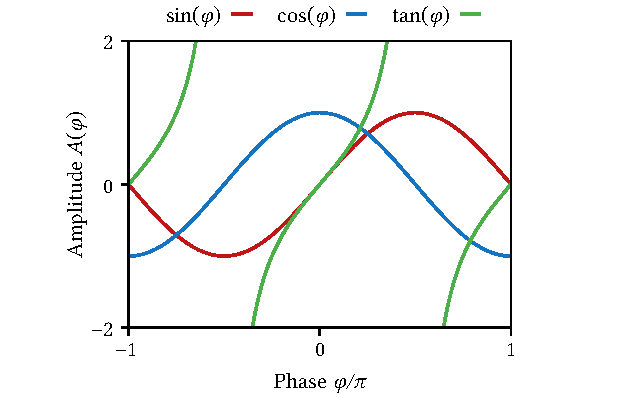
\includegraphics[width=0.2\textwidth]{test.jpg}
  \caption{This is simply a test figure, and some equation $\sin(2x)=1$, and some SI unit \SI{1.0e3}{m/s}, and some chemical \ce{CrO2}. This text can even be made even longer, since we want to test this properly.}
  \label{fig:test}
\end{figure}


Morbi non tortor volutpat, mattis odio at, tincidunt libero.
Donec pulvinar et mi at varius.
Sed vulputate lectus eu libero gravida, vel porta tortor bibendum.
Quisque dictum ex id quam ultrices, ut commodo nisl euismod.
Aliquam vulputate, urna quis sodales rhoncus, orci metus pulvinar velit, feugiat sollicitudin dui massa interdum tortor.
Nam sed ante vitae eros imperdiet bibendum.
Fusce pretium semper leo eget lobortis.
Sed dictum erat quis diam faucibus bibendum.
Integer vitae enim euismod, ornare augue quis, pharetra ante.
Phasellus venenatis tellus ut velit faucibus, posuere porttitor lacus hendrerit.

\begin{table}[h!]
  \centering
  \caption{This is simply a test table.}
  \label{tab:test}
  \begin{tabular*}{\dimexpr\textwidth-4em\relax}{@{\extracolsep{\stretch{1}}\,}lcc@{\,}}
    \toprule
    Name    &   Symbol    &   Value             \\
    \midrule
    Euler constant          & $e$   & $2.71...$  \\
    Circle constant         & $\pi$ & $3.14...$ \\
    Imaginary identity      & $i$ & $\sqrt{-1}$ \\
    \bottomrule
  \end{tabular*}
\end{table}

Lorem ipsum dolor sit amet, consectetur adipiscing elit.
Donec malesuada magna sem.
Fusce vitae lectus id magna convallis euismod.
Quisque viverra sollicitudin turpis, vel ultricies mauris dictum quis.
Praesent justo nunc, luctus in lectus in, placerat tempus orci.
Donec placerat neque ac tortor dignissim pellentesque.
Aenean tellus erat, eleifend id interdum a, volutpat et massa.
Quisque tristique accumsan efficitur.

Morbi non tortor volutpat, mattis odio at, tincidunt libero.
Donec pulvinar et mi at varius.
Sed vulputate lectus eu libero gravida, vel porta tortor bibendum.
Quisque dictum ex id quam ultrices, ut commodo nisl euismod.
Aliquam vulputate, urna quis sodales rhoncus, orci metus pulvinar velit, feugiat sollicitudin dui massa interdum tortor.
Nam sed ante vitae eros imperdiet bibendum.
Fusce pretium semper leo eget lobortis.
Sed dictum erat quis diam faucibus bibendum.
Integer vitae enim euismod, ornare augue quis, pharetra ante.
Phasellus venenatis tellus ut velit faucibus, posuere porttitor lacus hendrerit.

Lorem ipsum dolor sit amet, consectetur adipiscing elit.
Donec malesuada magna sem.
Fusce vitae lectus id magna convallis euismod.
Quisque viverra sollicitudin turpis, vel ultricies mauris dictum quis.
Praesent justo nunc, luctus in lectus in, placerat tempus orci.
Donec placerat neque ac tortor dignissim pellentesque.
Aenean tellus erat, eleifend id interdum a, volutpat et massa.
Quisque tristique accumsan efficitur.


\section{Continuation}
Morbi non tortor volutpat, mattis odio at, tincidunt libero.
Donec pulvinar et mi at varius.
Sed vulputate lectus eu libero gravida, vel porta tortor bibendum.
Quisque dictum ex id quam ultrices, ut commodo nisl euismod.
Aliquam vulputate, urna quis sodales rhoncus, orci metus pulvinar velit, feugiat sollicitudin dui massa interdum tortor.
Nam sed ante vitae eros imperdiet bibendum.
Fusce pretium semper leo eget lobortis.
Sed dictum erat quis diam faucibus bibendum.
Integer vitae enim euismod, ornare augue quis, pharetra ante.
Phasellus venenatis tellus ut velit faucibus, posuere porttitor lacus hendrerit.

Lorem ipsum dolor sit amet, consectetur adipiscing elit.\cite{feynman,statistics}\footnote{test}
Donec malesuada magna sem.
Fusce vitae lectus id magna convallis euismod.
Quisque viverra sollicitudin turpis, vel ultricies mauris dictum quis.
Praesent justo nunc, luctus in lectus in, placerat tempus orci.
Donec placerat neque ac tortor dignissim pellentesque.
Aenean tellus erat, eleifend id interdum a, volutpat et massa.
Quisque tristique accumsan efficitur.

Morbi non tortor volutpat, mattis odio at, tincidunt libero.
Donec pulvinar et mi at varius.
Sed vulputate lectus eu libero gravida, vel porta tortor bibendum.
Quisque dictum ex id quam ultrices, ut commodo nisl euismod.
Aliquam vulputate, urna quis sodales rhoncus, orci metus pulvinar velit, feugiat sollicitudin dui massa interdum tortor.\footnote{This is another footnote test.} %\footnote{This is simply just a simple test, with an equation $\sin \alpha = \cos(2a-1)/\cos(2a+1)$. And here is a chemical element \ce{CrO23} and physical unit \SI{12e3}{m}. }\footnote{Here is another footnote, also set in sans-serif.}%\footnote{$ABCDEFGHIJKLMOPQRSTUVWXYZ$ $abcdefghijklmopqrstuvwxyz$ $\alpha\beta\gamma\delta$ $\Gamma\Delta$ $\int_0^\infty \mathrm{d}x\,\sum_{ij} f(x_{ij}) \leq 0 \mathbf{xyz} \hat{x}+\check{y}\cdot\bar{u} \mathcal{F} \mathbf{x\sigma}$ $\sin x$  $\cos x$}
Nam sed ante vitae eros imperdiet bibendum. 
Fusce pretium semper leo eget lobortis.
Sed dictum erat quis diam faucibus bibendum.
Integer vitae enim euismod, ornare augue quis, pharetra ante.
Phasellus venenatis tellus ut velit faucibus, posuere porttitor lacus hendrerit.

Lorem ipsum dolor sit amet, consectetur adipiscing elit.
Donec malesuada magna sem.
Fusce vitae lectus id magna convallis euismod.
Quisque viverra sollicitudin turpis, vel ultricies mauris dictum quis.
Praesent justo nunc, luctus in lectus in, placerat tempus orci.
Donec placerat neque ac tortor dignissim pellentesque.
Aenean tellus erat, eleifend id interdum a, volutpat et massa.
Quisque tristique accumsan efficitur.

Morbi non tortor volutpat, mattis odio at, tincidunt libero.
Donec pulvinar et mi at varius.
Sed vulputate lectus eu libero gravida, vel porta tortor bibendum.
Quisque dictum ex id quam ultrices, ut commodo nisl euismod.
Aliquam vulputate, urna quis sodales rhoncus, orci metus pulvinar velit, feugiat sollicitudin dui massa interdum tortor.
Nam sed ante vitae eros imperdiet bibendum.
Fusce pretium semper leo eget lobortis.
Sed dictum erat quis diam faucibus bibendum.\footnote{Test}\cite{particle}
Integer vitae enim euismod, ornare augue quis, pharetra ante.
Phasellus venenatis tellus ut velit faucibus, posuere porttitor lacus hendrerit.


%
%\clearpage
%\chapter*{Bestemte integral}\noindent
%Under skal jeg prøve å gi en rask intro til bestemt integrasjon.
%Måten jeg gjør det på, er som følger: jeg kommer bare til å hoppe rett inn i det ved å demonstrere hvordan man løser to eksempeloppgaver.
%Etter det, skal jeg prøve å gi en kort oppsummering av hvordan man logisk kan tenke på bestemte integraler etterpå.
%Dette blir ikke en veldig dyp intro, men håper at det gir deg det du trenger for å løse eksamensoppgavene iallefall :).
%
%\section*{Eksempel I: introduksjon}\noindent
%La oss starte med et relativt enkelt eksempel på et bestemt integral:
%\begin{equation*}
%  \int_{x=0}^{x=1} x^2\,\text{d}x
%\end{equation*}
%Dette skrives ofte uten $x=\cdots$, altså på kortformen:
%\begin{equation*}
%  \int_{0}^{1} x^2\,\text{d}x
%\end{equation*}
%Når man skal løse et bestemt integral, må man alltid starte med å løse det ubestemte integralet.
%Hvis du slår opp i formelsamlingen bakerst i et av eksamenssettene, finner du en formel for ubestemte integral av polynomer:
%\begin{align*}
%  \int x^r\;\text{d}x &= \frac{1}{r+1} x^{r+1} & &\text{(for $r\neq-1$)}
%\end{align*}
%Setter du inn $r=2$ finner du da:
%\begin{align*}
%  \int x^2\;\text{d}x = \frac{1}{3} x^3
%\end{align*}
%Okay, la oss nå gå tilbake til det \emph{bestemte} integralet.
%Den vanlige måten å skrive ned at man har løst det \emph{ubestemte} integralet på, er å sette firkantklammer rundt svaret, med de såkallte \emph{integrasjonsgrensene} 0 og 1 utenfor klammene:
%\begin{equation*}
%  \int_{x=0}^{x=1} x^2\,\text{d}x = \left[ \frac{1}{3} x^3 \right]_{x=0}^{x=1}
%\end{equation*}
%Det å faktisk regne ut det bestemte integralet fra det ubestemte er nå veldig enkelt: vi trenger faktisk bare å sette inn $x=1$ og $x=0$ i det uttrykket som står i klammer, og så trekke svarene fra hverandre:
%\begin{align*}
%  \left[ \frac{1}{3} x^3 \right]_{x=0}^{x=1} 
%  &= \left[ \frac{1}{3} x^3 \right]_{x=1} - \;\;\;\;\left[ \frac{1}{3} x^3 \right]_{x=0} \\
%  &= \left[ \frac{1}{3} \cdot 1^3 \right]\;\;\; - \;\;\;\left[ \frac{1}{3} \cdot 0^3 \right] \\
%  &= \frac{1}{3} - 0 \\
%  &= \frac{1}{3}
%\end{align*}
%Svaret fra den bestemte integrasjonen blir altså:
%\begin{equation*}
%  \int_0^1 x^2\,\text{d}x = \frac{1}{3}
%\end{equation*}
%
%\section*{Eksempel II: avansert}
%Okay, la oss se på en litt mer avansert oppgave:
%\begin{equation*}
%  \int_1^\infty e^{-2x}
%\end{equation*}
%Første steg er som sagt alltid å løse det ubestemte integralet. 
%Sjekker du formelsamlingen bakerst i et eksamenssett dine, finner du denne likningen:
%\begin{align*}
%  \int e^{kx}\;\text{d}x &= \frac{1}{k} e^{kx} + C & &\text{($C$ er en vilkårlig konstant)}
%\end{align*}
%Sett inn at $k=-2$:
%\begin{align*}
%  \int e^{-2x}\;\text{d}x &= -\frac{1}{2} e^{-2x} + C
%\end{align*}
%Så løsningen på det ubestemte integralet er også:
%\begin{align*}
%  \int_{1}^{\infty} e^{-2x}\;\text{d}x &= \left[ -\frac{1}{2} e^{-2x} + C \right]_1^\infty
%\end{align*}
%Vi finner da løsningen på det bestemte integralet ved å sette inn $x=\infty$ og $x=1$, og trekke resultatene fra hverandre.
%En detalj som trengs her, er da at $e^{-\infty} = 1/e^{\infty} = 1/\infty = 0$; har du ikke lært om grenseverdier i faget, så trenger du ikke å tenke så mye på dette, det er isåfall muligens utenfor pensum :).
%Men beregningen blir altså:
%\begin{align*}
%  \int_{1}^{\infty} e^{-2x}\;\text{d}x 
%  &= \left[ -\frac{1}{2} e^{-2x}     + C \right]_1^\infty \\
%  &= \left[ -\frac{1}{2} e^{-2x}     + C \right]_{x=\infty} - \;\;\;\;\left[ -\frac{1}{2} e^{-2x} + C \right]_{x=1} \\
%  &= \left[ -\frac{1}{2} e^{-\infty} + C \right] \;\;\;\;\;\; - \;\;\;\; \left[ -\frac{1}{2} e^{-2} + C \right] \\
%  &= \left[ -\frac{1}{2} \cdot 0 \; +  C \right] \;\;\;\;\;\; - \;\;\;\; \left[ -\frac{1}{2} e^{-2} + C \right] \\
%  &= 0 + C + \frac{1}{2} e^{-2} - C \\
%  &= \frac{1}{2} e^{-2} \\
%  &= \frac{1}{2e^2}
%\end{align*}
%Så svaret er:
%\begin{align*}
%  \int_{1}^{\infty} e^{-2x}\;\text{d}x &= \frac{1}{2e^2}
%\end{align*}
%Merk at det ikke hadde noe å si at vi ikke visste hva den ukjente konstanten $C$ var for noe, den forsvant uansett når vi beregnet et bestemt integral :).
%
%\section*{Tolkning I: antiderivasjon}
%En måte å tolke hva integrasjon betyr for noe, er at det er \emph{det omvendte av derivasjon}. 
%For eksempel, hvis vi tar det ubestemte integralet vi så på over:
%\begin{align*}
%  \int x^2\;\text{d}x &= \frac{1}{3} x^{3}
%\end{align*}
%Hva skjer hvis vi deriverer svaret? 
%Jo, den deriverte av $x^{3}$ er $3x^2$, så vi får:
%\begin{align*}
%  \left( \int x^2\;\text{d}x \right)' &= x^{2}
%\end{align*}
%Så hvis vi først integrerer $x^2$ og så deriverer svaret, så får vi tilbake det vi startet med.
%Derivasjonen gjorde det motsatte av det integrasjonen gjorde.
%
%Hva betyr dette for hvordan vi skal tolke integrasjon?
%Jo, det derivasjon måler er jo \emph{stigningstallet} eller \emph{endringsraten} til noe.
%For eksempel, hvis du vet posisjonen $s$ til en bil som funksjon av tiden $t$, så vil den deriverte $v(t) = s'(t)$ være \emph{hastigheten} til bilen.
%Siden integrasjon gjør det motsatte, betyr det at du kan integrere hastigheten for å finne ut hvor langt bilen faktisk har kjørt.
%
%
%\section*{Tolkning II: areal under en kurve}
%En geometrisk tolkning av integrasjon, er at det er en måte å regne ut arealet under en kurve.
%La oss f.eks. si at vi har en graf av funksjonen $f(x) = 1-x^2$:\\
%{\quad \includegraphics[width=0.6\textwidth]{/home/jabirali/figure.png}} \\
%Hvis vi tar et bestemt integral av denne funksjonen fra $x=0$ til $x=1$:
%\begin{equation*}
%  \int_0^1 (1-x^2)\;\text{d}x = \left[ x - \frac{1}{3}x^3 \right]_0^1 = [1 - 1/3] - [0 - 0] = 2/3
%\end{equation}
%Egentlig bare arealet under kurven mellom $x=0$ og $x=1$:\\
%{\quad \includegraphics[width=0.6\textwidth]{/home/jabirali/areal.png}}\\
%Det å \emph{bevise} at integraler gir deg areal er litt mer jobb, og sannsynligvis ikke verdt å fokusere på fram mot eksamen.
%Men det er greit å ha i bakhodet at hvis det kommer en eksamensoppgave hvor de vil at du skal ``finne arealet under kurven'', så betyr det bare at du skal løse et bestemt integral ;).
%
%Det at ``integral'' betyr ``areal under kurve'' gir jo en innsikt til.
%Et ``bestemt integral fra $x=0$ til $x=1$'' er altså arealet under kurven mellom punktene $x=0$ og $x=1$.
%Et ``ubestemt integral'' derimot, hvor vi ikke har satt inn noen verdier for $x$ enda, er en generell formel for å regne ut arealet under kurven for vilkårlige startpunkt og sluttpunkt.
%Dette minner jo litt om den samme situasjonen for derivasjon: $f'(x)$ er en ``ubestemt derivert'', altså en generell formel for å regne ut stigningstall. Hvis du setter inn $x=2$ i dette uttrykket, altså beregner $f'(2)$, så har du derimot spesifikt stigningstallet til kurven i punktet $x=2$, som vi godt kunne kallt en ``bestemt derivert''.





    %\chapter{Introduction}
Blah.
 
    %\chapter{Quasiclassical theory}
In here: define notation, propagators, and matrix current.
Make it clear what approximations we have performed.

\section{Propagators}
\section{Matrix current}
%Usadel diffusion equation:
%\begin{equation}
%  iD \nabla\cdot\mathbf{I} = U 
%\end{equation}
%Boundary conditions:
%\begin{equation}
%  \mathbf{I}_a = \mathbf{I}_b = [g_a, g_b]
%\end{equation}

\section{Novel notation}
Regarding the notation... How about simply saying fuck special notation for spin and nambu space? I mean, the reason we're having problems with overnotation is:
\begin{itemize}
  \item 2×2 matrices in spin space has underline-notation;
  \item 2×2 matrices in nambu space has hat-notation;
  \item 4×4 matrices in spin-nambu space has underline+hat notation;
  \item 8-element vectors in our rho-space has vec notation;
  \item The resulting 8×4×4 basis vector $\rho$ should get vec+underline+hat notation;
  \item We haven't chosen a notation for 8×8 matrices in rho-space yet...
\end{itemize}
And so on. It becomes chaos, and at this point, all the extra notation will rather serve to confuse the reader than help the reader grok what we're doing. Also,
the more special notation of this kind, the larger the risk of mistakes -- and a single mistake in all of these hats and underlines will cause a lot of confusion for the reader.

So how about this: we drop as much annotation as possible, and just use explicit definitions instead, like explicitly saying "we define the 8-element vector..." or "define the 8×8 matrix" etc instead of implying this from notation.

First of all, fuck non-quasiclassical quantities. All our equations are quasiclassical anyway, so we might as well not reserve e.g. $\check{G}$ for the non-quasiclassical propagator. 
So we define the Green's function etc as:
\begin{align}
\bm{G} &= \begin{bmatrix}\bm{G}^R & \bm{G}^K \\ 0 & \bm{G}^A \end{bmatrix}, &
\bm{J} &= \begin{bmatrix}\bm{J}^R & \bm{J}^K \\ 0 & \bm{J}^A \end{bmatrix}, &
\bm{U} &= \begin{bmatrix}\bm{U}^R & \bm{U}^K \\ 0 & \bm{U}^A \end{bmatrix}.
\end{align}
No underline, no check, no hat. Just bold letters, with a superscript that mentions R/K/A as usual.
Then we use lower-case letters for the spin-space decomposition:
\begin{align}
\bm{G}^R &= \begin{bmatrix}+\bm{g}^R & +\bm{f}^R \\ -\tilde{\bm{f}}^R & -\tilde{\bm{f}}^R \end{bmatrix}, &
\bm{J}^R &= \begin{bmatrix}+\bm{j}^R & +\bm{i}^R \\ -\tilde{\bm{i}}^R & -\tilde{\bm{j}}^R \end{bmatrix}, &
\bm{U}^R &= \begin{bmatrix}+\bm{u}^R & +\bm{v}^R \\ -\tilde{\bm{v}}^R & -\tilde{\bm{u}}^R \end{bmatrix}. &
\end{align}
When we define these, we explicitly say that all the lower-case quantities are 2×2 matrices in spin-space.
Then we explicitly define the rhos as:
\begin{align*}
  \bm\rho_0 &= \text{diag}(+\bm\sigma_0, +\bm\sigma_0^*), &
  \bm\rho_4 &= \text{diag}(+\bm\sigma_0, -\bm\sigma_0^*), \\
         &\;\;\vdots                             &
         &\;\;\vdots                             \\
  \bm\rho_3 &= \text{diag}(+\bm\sigma_3, +\bm\sigma_3^*), &
  \bm\rho_7 &= \text{diag}(+\bm\sigma_3, -\bm\sigma_3^*), \\
\end{align*}
where we mention that $\sigma_0$ is the identity and $\sigma_n$ the 2×2 Pauli matrices.
Then we say that we group these into an 8-element vector:
\begin{equation}
  \vec{\bm\rho} = [\bm\rho_0, \ldots, \bm\rho_7]
\end{equation}
At this point, we introduce a single new notation: things with a vector arrow have a structure in the 8-dimension spin-nambu vector space defined here.
We then define the new notation for the distribution function and currents in this new space:
\begin{align}
  \bm{H} &= \vec{H} \cdot \vec{\bm{\rho}}, &
  \bm{J} &= \vec{J} \cdot \vec{\bm{\rho}}.
\end{align}
So we dot two vector quantities, namely the 8-element vector and the 8×4×4-element basis vector, and get a 4×4-element matrix out.
No bold for the 8-element vectors, as they're in a different space.
I'm using a capital letter for the distribution function to follow the implicit ``lower-case letters are spin-space'' logic.
The inverse transformation is:
\begin{align}
  \vec{H} &= \text{Tr}[ \bm{H} \vec{\bm{\rho}} ] / 4, &
  \vec{J} &= \text{Tr}[ \bm{J} \vec{\bm{\rho}} ] / 4
\end{align}
So we "trace away" the matrix structure to map the distribution function onto our 8-element vector space.
Once we have two 8-element vector quantities, we define an 8×8 relationship between them using tensor notation:
\begin{align}
  \vec{J} = \tensor{M} \vec{H}
\end{align}

    %\chapter{Diffusion equation}
Usadel.

    %\chapter{Kinetic equation}
\section{Introduction}
After we perform a Pauli-decomposition, the part of the Usadel equation describing the nonequilibrium distribution function~$\BC{H}$ -- also known as the \emph{kinetic equation} -- can be written [Eq.~(12) in our arXiv manuscript]:
\begin{equation}
  \BC{U} = -\partial_z \BC{J}
\end{equation}
Meanwhile, the nonequilibrium matrix current becomes [Eq.~(21)]:
\begin{equation}
  \BC{J} = \BC{M}\partial_z\BC{H} + \BC{Q}\BC{H}
\end{equation}
Substituting the latter into the former we get [Eq.~(39)]:
\begin{equation}
  \BC{M} \partial_z^2 \BC{H} = -\big[ (\partial_z\BC{M}) + \BC{Q} \big] \partial_z \BC{H} - (\partial_z \BC{Q}) \BC{H} - \BC{U}
\end{equation}
What I will show here, is that we can in general write $\BC{U} = \BC{K} \BC{H}$, so that:
\begin{equation}
  \BC{M} \partial_z^2 \BC{H} = -\big[ (\partial_z\BC{M}) + \BC{Q} \big] \partial_z \BC{H} - \big[ (\partial_z \BC{Q}) + \BC{K} \big] \BC{H}
\end{equation}
If we then define the quantities:
\begin{align}
  \BC{C}_1 &= -\BC{M}^{-1} \big[ (\partial_z\BC{M}) + \BC{Q} \big] \\
  \BC{C}_2 &= -\BC{M}^{-1} \big[ \, (\partial_z\BC{Q}) \,+ \BC{K} \big]
\end{align}
Then the kinetic equation can be written simply as:
\begin{equation}
  \partial_z^2 \BC{H} = \BC{C}_1 \partial_z \BC{H} + \BC{C}_2 \BC{H}
\end{equation}
Here, the matrices $\BC{C}_1$ and $\BC{C}_2$ are determined solely by equilibrium properties, and thus can be considered constants when solving the nonequilibrium equation above.
This should make this form of the equation very efficient to solve, since it is an \emph{explicit and linear differential equation}.

\clearpage
\section{First-order terms}
First, I will look at terms which are first-order in the $8\times8$ propagator~$\UV{G}$.
Before Pauli-decomposition, the Usadel equation for such terms look like
\begin{equation}
  iD \partial_z(\UV{G} \partial_z \UV{G}) = \big[ \UV{\Sigma}, \UV{G} \big],
\end{equation}
where I first assume that $\UV{\Sigma}$ is independent of $\UV{G}$, making the right-hand side above first-order in $\UV{G}$.
Upon introducing $\UV{I} \sim \UV{G} \partial_z \UV{G}$ and $\UV{U} \sim \big[ \UV{\Sigma}, \UV{G} \big]$, we get
\begin{equation}
  \partial_z \UV{I} = \UV{U}.
\end{equation}
Writing out the Keldysh-space structure, the potential $\UV{U}$ becomes
\begin{align}
  \UV{U} &=
    \begin{pmatrix}
      \U\Sigma & 0 \\[0.5ex]
      0 & \U\Sigma
    \end{pmatrix}
    \begin{pmatrix}
      {\U G}^R & {\U G}^K \\[0.5ex]
      0        & {\U G}^A
    \end{pmatrix}
    -
    \begin{pmatrix}
      {\U G}^R & {\U G}^K \\[0.5ex]
      0        & {\U G}^A
    \end{pmatrix}
    \begin{pmatrix}
      \U\Sigma & 0 \\[0.5ex]
      0 & \U\Sigma
    \end{pmatrix}
  \\ &=
    \begin{pmatrix}
      \big[{\U\Sigma}\big, {\U G}^R] & \big[{\U\Sigma}, {\U G}^K\big] \\[1ex]
      0        & \big[{\U\Sigma}, {\U G}^A\big]
    \end{pmatrix}
\end{align}
In other words, as long as the self-energy is diagonal in Keldysh space, the Keldysh component of the matrix potential is simply
\begin{equation}
  {\U U}^K = \big[ {\U\Sigma}, {\U G}^K \big] .
\end{equation}
Now, the Pauli-decompositions of the Kelydysh components were:
\begin{align}
  \C{J}_i & \equiv \frac{1}{4} \tr\left\{ {\U \rho_i} {\U I}^K \right\}, &
  \C{U}_i & \equiv \frac{1}{4} \tr\left\{ {\U \rho_i} {\U U}^K \right\}.
\end{align}
Using the above equation for ${\U U}^K$ and the cyclic rule for traces:
\begin{align}
  \C{U}_i 
  &= \frac{1}{4} \tr\left\{ {\U \rho_i} \big[ {\U\Sigma}, {\U G}^K\big] \right\} \\
  &= \frac{1}{4} \tr\left\{ {\U \rho_i} \big[ {\U\Sigma} {\U G}^K - {\U G}^K {\U\Sigma} \big] \right\} \\
  &= \frac{1}{4} \tr\left\{ {\U \rho_i} {\U\Sigma} {\U G}^K - {\U\Sigma} {\U \rho_i} {\U G}^K \right\} \\
  &= \frac{1}{4} \tr\left\{ \big[{\U \rho_i}, {\U\Sigma}\big] {\U G}^K \right\}.
\end{align}
Inserting ${\U G}^K = {\U G}^R {\U H} - {\U H} {\U G}^A$:
\begin{align}
  \C{U}_i 
  &= \frac{1}{4} \tr\left\{ \big[{\U \rho_i}, {\U\Sigma}\big] {\U G}^R {\U H} - \big[{\U \rho_i}, {\U\Sigma}\big] {\U H} {\U G}^A \right\} \\
  &= \frac{1}{4} \tr\left\{ \big[{\U \rho_i}, {\U\Sigma}\big] {\U G}^R {\U H} - {\U G}^A \big[{\U \rho_i}, {\U\Sigma}\big] {\U H} \right\}.
\end{align}
As we did for the Pauli-decomposition of the current and potential, we can insert $\U H = \sum_j \C{H}_j {\U \rho}_j$, and move the scalar coefficients $\C{H}_j$ and summation out of the trace.
What we find then, is that the equation above can be written
\begin{align}
  \C{U}_i = \sum_j \C{K}_{ij} \C{H}_j,
\end{align}
where we define the new matrix coefficient
\begin{align}
  \C{K}_{ij}
  &= \frac{1}{4} \tr\left\{ \big[{\U \rho_i}, {\U\Sigma}\big] {\U G}^R {\U \rho}_j - {\U G}^A \big[{\U \rho_i}, {\U\Sigma}\big] {\U \rho}_j \right\}.
\end{align}
There are two things to note about this result.
First, this equation makes it almost trivial to specify the Usadel equation for new materials, since it is a direct function of the self-energy $\U \Sigma$ that we would put into the Usadel equation itself.
Second, the matrix $\U \Sigma$ is just filled with system parameters that we set (energy, exchange field, etc.), while the matrices ${\U G}^R$ and ${\U G}^A$ only depend on the equilibrium solution.
Since this matrix is completely independent of the nonequilibrium distribution $\BC H$, we can precalculate it before solving the differential equation, and do not have to evaluate it more than once per energy and position.



\section{Second-order terms}
Above, we considered a matrix potential $\V{U} = \big[\V{\Sigma}, \V{G}\big]$ where $\V{\Sigma}$ assumed to be independent of $\V{G}$.
This is sufficient for a lot of systems (e.g. normal metals, ferromagnets, even half-metals), but not completely general.
There are at least three exceptions I know of based on the projects I've worked on so far:\\[1ex]
\begin{tabular}{ll}
  Spin-flip scattering: &
  $\V{U} \sim \big[ \tau_3 \BU{\sigma} \V{G} \BU{\sigma} \tau_3, \V{G} \big];$ \\[0.5ex]
  Spin-orbit scattering: &
  $\V{U} \sim \big[ \phantom{\tau_3}\BU{\sigma} \V{G} \BU{\sigma} \phantom{\tau_3}, \V{G} \big];$ \\[0.5ex]
  Orbital depairing: & 
  $\V{U} \sim \big[  \tau_3 \phantom{\BU{\sigma}}\V{G} \phantom{\BU{\sigma}} \tau_3 , \V{G} \big]$.\\[1ex]
\end{tabular}

\noindent
Note that all of the above are second-order in the propagator~$\V{G}$, and has the same basic structure $\V{U} = \big[ \V{\Sigma} \V{G} \V{\Sigma}, \V{G} \big]$.
The matrix $\V{\Sigma}$ in this expression is again diagonal in Keldysh space and independent of the propagator $\V{G}$.
Let us now check what happens if we assume such a form for the potential~$\V{U}$:
\begin{align*}
  \UV{U}
  &=
    \big[ \V{\Sigma} \V{G} \V{\Sigma}, \V{G} \big] 
  \\ &=
    \begin{pmatrix}
      {\U\Sigma} {\U G}^R {\U\Sigma} &
      {\U\Sigma} {\U G}^K {\U\Sigma} \\
      0                              &
      {\U\Sigma} {\U G}^A {\U\Sigma} 
    \end{pmatrix}
    \begin{pmatrix}
      {\U G}^R & {\U G}^K \\[0.5ex]
      0        & {\U G}^A
    \end{pmatrix}
    -
    \begin{pmatrix}
      {\U G}^R & {\U G}^K \\[0.5ex]
      0        & {\U G}^A
    \end{pmatrix}
    \begin{pmatrix}
      {\U\Sigma} {\U G}^R {\U\Sigma} &
      {\U\Sigma} {\U G}^K {\U\Sigma} \\
      0                              &
      {\U\Sigma} {\U G}^A {\U\Sigma} 
    \end{pmatrix}
  \\ &=
    \begin{pmatrix}
      \big[{\U\Sigma} {\U G}^R {\U\Sigma}\big, {\U G}^R] & 
      {\U\Sigma} {\U G}^R {\U\Sigma} {\U G}^K            +
      {\U\Sigma} {\U G}^K {\U\Sigma} {\U G}^A            - 
      {\U G}^R {\U\Sigma} {\U G}^K {\U\Sigma}            -
      {\U G}^K {\U\Sigma} {\U G}^A {\U\Sigma}            \\[1ex]
      0                                                  &
      \big[{\U\Sigma} {\U G}^A {\U\Sigma}, {\U G}^A\big]
    \end{pmatrix}
\end{align*} 
In other words, the Keldysh component takes the more complicated form:
\begin{equation}
  \U{U}^K = 
      {\U\Sigma} {\U G}^R {\U\Sigma} {\U G}^K +
      {\U\Sigma} {\U G}^K {\U\Sigma} {\U G}^A - 
      {\U G}^R {\U\Sigma} {\U G}^K {\U\Sigma} -
      {\U G}^K {\U\Sigma} {\U G}^A {\U\Sigma} .
\end{equation}
Like before, we can multiply by ${\U\rho}_i$ and trace to obtain the Pauli-decomposition, then use the cyclic trace rule and reorder the terms a bit:
\begin{align*}
  \C{U}_i
  &= 
    \frac{1}{4}
    \tr 
    \left\{
      {\U\rho}_i {\U\Sigma} {\U G}^R {\U\Sigma} {\U G}^K +
      {\U\rho}_i {\U\Sigma} {\U G}^K {\U\Sigma} {\U G}^A - 
      {\U\rho}_i {\U G}^R {\U\Sigma} {\U G}^K {\U\Sigma} -
      {\U\rho}_i {\U G}^K {\U\Sigma} {\U G}^A {\U\Sigma} 
    \right\}
  \\ 
  &= 
    \frac{1}{4}
    \tr 
    \left\{
      {\U\rho}_i {\U\Sigma} {\U G}^R {\U\Sigma} {\U G}^K +
      {\U\Sigma} {\U G}^A {\U\rho}_i {\U\Sigma} {\U G}^K - 
      {\U\Sigma} {\U\rho}_i {\U G}^R {\U\Sigma} {\U G}^K -
      {\U\Sigma} {\U G}^A {\U\Sigma} {\U\rho}_i {\U G}^K 
    \right\}
  \\ 
  &= 
    \frac{1}{4}
    \tr 
    \left\{
      \big[ {\U\rho}_i, {\U\Sigma} \big] {\U G}^R {\U\Sigma} {\U G}^K +
      {\U\Sigma} {\U G}^A \big[ {\U\rho}_i, {\U\Sigma} \big] {\U G}^K 
    \right\}
\end{align*}
For simplicity, let's write this in the following form for now:
\begin{align}
  \C{U}_i
  &= 
    \frac{1}{4} \tr \left\{ \U F_i {\U G}^K \right\}
  ,
  &
  \U F_i
  = \big[ {\U\rho}_i, {\U\Sigma} \big] {\U G}^R {\U\Sigma} 
  + {\U\Sigma} {\U G}^A \big[ {\U\rho}_i, {\U\Sigma} \big]
  .
\end{align}
We then substitute in ${\U G}^K = {\U G}^R {\U H} - {\U H} {\U G}^A$:
\begin{align}
  \C{U}_i
  = 
    \frac{1}{4}
    \tr 
    \left\{
      {\U F}_i {\U G}^R {\U H} -
      {\U F}_i {\U H} {\U G}^A 
    \right\}
  = 
    \frac{1}{4}
    \tr 
    \left\{
      {\U F}_i {\U G}^R {\U H} -
      {\U G}^A {\U F}_i {\U H}
    \right\}
\end{align}
We then use $\U H = \sum_j H_j {\U\rho}_j$ to write the above equation as:
\begin{align}
  \C{U}_i    &= \sum_j \C{K}_{ij} \C{H}_j, &
  \C{K}_{ij} &= \frac{1}{4} \tr \left\{ {\U F}_i {\U G}^R {\U\rho}_j - {\U G}^A {\U F}_i {\U \rho}_j \right\}.
\end{align}
We could substitute back the definition of ${\U F}_i$ to see the explicit form of $\C{K}_{ij}$:
\begin{align*}
  \C{K}_{ij} = 
  \frac{1}{4} \tr 
  \Big\{
  &   \big[ {\U\rho}_i, {\U\Sigma} \big] {\U G}^R {\U\Sigma} {\U G}^R {\U\rho}_j
    + {\U\Sigma} {\U G}^A \big[ {\U\rho}_i, {\U\Sigma} \big] {\U G}^R {\U\rho}_j \\
  & - {\U G}^A \big[ {\U\rho}_i, {\U\Sigma} \big] {\U G}^R {\U\Sigma} {\U \rho}_j
    - {\U G}^A {\U\Sigma} {\U G}^A \big[ {\U\rho}_i, {\U\Sigma} \big] {\U \rho}_j
  \Big\}
\end{align*}
This expression has some symmetries.
Let us use the cyclic trace rule to rewrite it such that the commutator $\big[ {\U\rho}_i, {\U\Sigma} \big]$ comes first in each term:
\begin{align*}
  \C{K}_{ij} = 
  \frac{1}{4} \tr 
  \Big\{
  &   \big[ {\U\rho}_i, {\U\Sigma} \big] {\U G}^R {\U\Sigma} {\U G}^R {\U\rho}_j
    + \big[ {\U\rho}_i, {\U\Sigma} \big] {\U G}^R {\U\rho}_j {\U\Sigma} {\U G}^A \\
  & - \big[ {\U\rho}_i, {\U\Sigma} \big] {\U G}^R {\U\Sigma} {\U \rho}_j {\U G}^A
    - \big[ {\U\rho}_i, {\U\Sigma} \big] {\U \rho}_j {\U G}^A {\U\Sigma} {\U G}^A
  \Big\}
\end{align*}
It then becomes clear that this commutator can be factored out of all terms.
Furthermore, we see that the terms proportional to ${\U G}^R \cdots {\U G}^A$ have a commutator structure.
Thus, the above may be simplified to:
\begin{align*}
  \C{K}_{ij} = 
  \frac{1}{4} \tr 
  \Big\{
      \big[ {\U\rho}_i, {\U\Sigma} \big]
      \left( 
        {\U G}^R {\U\Sigma} {\U G}^R {\U\rho}_j
      - {\U \rho}_j {\U G}^A {\U\Sigma} {\U G}^A
      + {\U G}^R \big[{\U \rho}_j, {\U\Sigma} \big] {\U G}^A
      \right)
  \Big\}
\end{align*}
This solves the problem of second-order terms $\UV{U} \sim \big[\UV{\Sigma}\UV{G}\UV{\Sigma}, \UV{G}\big]$.

\section{Summary}
If we have a very general Usadel equation of the form:
\begin{align}
  iD \partial_z(\UV{G} \partial_z \UV{G}) = \big[ \UV{\Sigma}^{(1)} + \UV{\Sigma}^{(2)}\UV{G}\UV{\Sigma}^{(2)}, \UV{G} \big],
\end{align} 
I have shown that the Pauli-decomposed Usadel equation may be written:
\begin{equation}
  \BC{M} \partial_z^2 \BC{H} = -\big[ (\partial_z\BC{M}) + \BC{Q} \big] \partial_z \BC{H} - \big[ (\partial_z \BC{Q}) + \BC{K} \big] \BC{H}
\end{equation}
Where the contributions to $\BC{K}$ from the $\UV{\Sigma}^{(1)}$ and $\UV{\Sigma}^{(2)}$ terms are given by:
\begin{align*}
  \C{K}_{ij}^{(1)}
  &= 
  \frac{1}{4} \tr\left\{ \big[{\U \rho_i}, {\U\Sigma}^{(1)}\big] \left({\U G}^R {\U \rho}_j - {\U \rho}_j {\U G}^A\right) \right\},
  \\
  \C{K}_{ij}^{(2)}
  &= 
  \frac{1}{4} \tr 
  \Big\{
      \big[ {\U\rho}_i, {\U\Sigma}^{(2)} \big]
      \left( 
        {\U G}^R {\U\Sigma}^{(2)} {\U G}^R {\U\rho}_j
      - {\U \rho}_j {\U G}^A {\U\Sigma}^{(2)} {\U G}^A
      + {\U G}^R \big[{\U \rho}_j, {\U\Sigma}^{(2)} \big] {\U G}^A
      \right)
  \Big\}.
\end{align*}
Note that since these matrices $\BC{Q}$, $\BC{M}$, and $\BC{K}$ are all completely independent of the nonequilibrium distribution function $\BC{H}$ and its derivatives, these can be precomputed from the equilibrium solution.
In other words, the final version of the kinetic equation can be written:
\begin{equation}
  \partial_z^2\BC{H} = \BC{C}_1 \partial_z \BC{H} + \BC{C}_2 \BC{H},
\end{equation}
where $\BC{C}_1$ and $\BC{C}_2$ are straight-forward to compute from the self-energies ${\UV\Sigma}^{(1)}$ and ${\UV\Sigma}^{(2)}$ and equilibrium propagators ${\UV G}^R$ and ${\UV G}^A$, and these coefficients only need to be computed once.
This yields an explicit linear differential equation for $\BC{H}$, which can be solved very efficiently numerically, and which should also be relatively simple to implement.
In its current form, the equation above will likely be even faster to solve than the Riccati-parametrized Usadel equation for the retarded propagator.

\clearpage
\section{Numerics}
We had reformulated the differential equation as:
\begin{equation}
  \partial_z^2\BC{H} = \BC{C}_1 \partial_z \BC{H} + \BC{C}_2 \BC{H}.
\end{equation}
This can be written as a first-order ordinary differential equation:
\begin{equation}
  \frac{d}{dz}
  \begin{pmatrix}
    \!\phantom{'}\BC{H}'\, \\
    \!\BC{H}\,
  \end{pmatrix}
  = 
  \begin{pmatrix}
    \BC{C}_1 & \BC{C}_2 \\
    1        & 0
  \end{pmatrix}
  \begin{pmatrix}
    \!\phantom{'}\BC{H}' \\
    \!\BC{H}
  \end{pmatrix}
\end{equation}
Note that this gives us an explicit form for the Jacobian, which can be provided directly to the boundary value problem solver.




\clearpage
\chapter{Physical observables}
\section{Introduction}
My equilibrium simulation program supports the calculation of the following physical observables:
  selfconsistent superconducting gap;
  charge and spin supercurrents;
  singlet/triplet decomposition of these currents;
  induced magnetization;
  and density of states.
Now that we are moving to nonequilibrium simulations, these equations need to be generalized.

First of all, the selfconsistency equation for the superconducting gap needs to be replaced with a version that depends on the nonequilibrium distribution.
The supercurrent equations need to be replaced with nonequilbrium versions, and in addition, we wish to calculate resistive currents now.
The induced magnetization needs to be supplemented with nonequilibrium charge and spin accumulation.
Furthermore, in nonequilibrium systems we might want to calculate heat currents and heat accumulation too.
Finally, since we're already rewriting a lot of the code for physical observables anyway, we might as well implement support for the spin-polarization of the density of states as well, which could be useful in the theoretical analysis.

This leaves one unaddressed point in the list above: the singlet/triplet decomposition of the charge current.
I believe that such a decomposition should still be possible in a general nonequilibrium setting, however Morten's current derivation assumes an equilibrium distribution function, and a nonequilibrium generalization would be more complex.
I therefore won't generalize this equation to nonequilibrium for now, but we can get back to this in the future if it turns out that we'll need it.

On the next pages, I'll write down the equations needed to consider all the points above theoretically, which I intend to implement numerically.
For now, I ignore the presence of spin-orbit coupling, which means that the equations for the currents will not be completely general, but they should be general enough to describe the spin-current project that we will be working on.
In the future, we can generalize these results if we need it for a spin-orbit coupled project, which should in practice only mean that we need to add a couple of new terms to the definition of the $\BC{M}$ and $\BC{Q}$ matrices in the code.



\clearpage
\section{Matrix current}
The full $8\times8$ matrix current is given by the expression:
\begin{align}
  \UV{I} 
  &= 
  \UV{G} \nabla \UV{G}
  \\ &= 
  \begin{pmatrix} 
    \U{G}^R  & \U{G}^K \\[1ex] 0 & \U{G}^A
  \end{pmatrix}
  \begin{pmatrix} 
    \nabla\U{G}^R  & \nabla\U{G}^K \\[1ex] 0 & \nabla\U{G}^A
  \end{pmatrix}
  \\ &= 
  \begin{pmatrix} 
    \U{G}^R\nabla\U{G}^R  & \U{G}^R\nabla\U{G}^K + \U{G}^K\nabla\U{G}^A \\[1ex] 0 & \U{G}^A\nabla\U{G}^A
  \end{pmatrix}
\end{align}
So the Keldysh component of the matrix current is:
\begin{align}
  \U{I}^K = \U{G}^R\nabla\U{G}^K + \U{G}^K\nabla\U{G}^A
\end{align}
Let us now substitute in $\U{G}^K = \U{G}^R \U{H} - \U{H} \U{G}^A$:
\begin{align*}
  \U{I}^K 
  &= 
  \U{G}^R\nabla(\U{G}^R \U{H} - \U{H} \U{G}^A)+ (\U{G}^R \U{H} - \U{H} \U{G}^A) \nabla\U{G}^A 
  \\ &=
  \U{G}^R(\nabla\U{G}^R) \U{H} + \U{G}^R\U{G}^R (\nabla\U{H}) - \U{G}^R (\nabla\U{H}) \U{G}^A 
  \\ &
  - \U{G}^R \U{H} (\nabla\U{G}^A) + \U{G}^R \U{H}(\nabla\U{G}^A) - \U{H} \U{G}^A (\nabla\U{G}^A)
  \\ &=
  \big[ (\U{G}^R \nabla \U{G}^R) \U{H} - \U{H} (\U{G}^A \nabla \U{G}^A) \big]
  \\ &\,+
  \big[ (\nabla\U{H}) - \U{G}^R (\nabla\U{H}) \U{G}^A \big]
\end{align*}
Let us give these two contributions to $\U{I}^K$ separate names:
\begin{align}
  \U{S}\, &\equiv (\U{G}^R \nabla \U{G}^R) \U{H} - \U{H} (\U{G}^A \nabla \U{G}^A),  \\
  \U{R}\, &\equiv (\nabla\U{H}) - \U{G}^R (\nabla\U{H}) \U{G}^A.
\end{align}
The first contribution $\U{S}$ is the \emph{supercurrent contribution} to the matrix current, which is independent of any potential gradients $\nabla\U{H}$, and can be nonzero even in equilibrium.
This is the matrix current equivalent to what Chandrasekhar and Tom called $\BC{Q}\BC{H}$.
As for the second contribution $\U{R}$, this is the \emph{resistive contribution} to the matrix current, which is only present when we have a potential gradient $\nabla\U{H}$.
This is what Chandrasekhar and Tom called $\BC{M}\nabla\BC{H}$.

\clearpage
\section{Energy symmetries}
In this section, I point out some new symmetries I noticed in the propagators, which will be useful to simplify the results derived in the following sections.
First, let us write out the structure of the propagators and distribution:
\begin{align}
  \U{G}^R &= 
  \begin{pmatrix}
    +\U{g}^R  & +\U{f}^R  \\[1ex]
   -\TU{f}^R & -\TU{g}^R
  \end{pmatrix} \\
  \U{G}^A &= 
  \begin{pmatrix}
    +\U{g}^A  & +\U{f}^A  \\[1ex]
   -\TU{f}^A & -\TU{g}^A
  \end{pmatrix} \\
  \U{G}^K &= 
  \begin{pmatrix}
    +\U{g}^K  & +\U{f}^K  \\[1ex]
   +\TU{f}^K & +\TU{g}^K
  \end{pmatrix} \\
  \U{H} \;&= \;
  \begin{pmatrix}
    \PM\U{h}  & \PM0\PM  \\[1ex]
    \PM0      & -\TU{h}\PM
  \end{pmatrix}
\end{align}
By explicit calculations, one can show that multiplying by $\N{1}$ from the left is equivalent to permuting rows, while multiplying by $\N{1}$ from the right permutes columns.
If we do both, we see from the structures above that:
\begin{align}
  \N{1} \U{G}^R \N{1}   &= -\TU{G}^R \\
  \N{1} \U{G}^A \N{1}   &= -\TU{G}^A \\
  \N{1} \U{G}^K \N{1}   &= +\TU{G}^K \\
  \N{1} \,\U{H}\, \N{1} &= -\TU{H}
\end{align}
Since tilde-conjugating is per definition a combination of complex conjugation $i \rightarrow -i$ and energy reversal $\epsilon \rightarrow -\epsilon$, this means that we get some simple identities relating the positive- and negative-energy propagators:
\begin{align}
  \U{G}^R(-\epsilon) &= -\N{1}\U{G}^{R*}(+\epsilon)\,\N{1} \\
  \U{G}^A(-\epsilon) &= -\N{1}\U{G}^{A*}(+\epsilon)\,\N{1} \\
  \U{G}^K(-\epsilon) &= +\N{1}\U{G}^{K*}(+\epsilon)\,\N{1} \\
  \U{H}(-\epsilon)   &= -\N{1}\U{H}^{*}(+\epsilon) \,\N{1}
\end{align}
If we substitute this into the matrix currents from the previous section:
\begin{align}
  \U{I}^K(-\epsilon) &= -\N{1} \U{I}^{K*}(+\epsilon)\N{1}, \\
  \U{S}(-\epsilon)\, &= -\N{1} \U{S}^*(+\epsilon)\, \N{1}, \\
  \U{R}(-\epsilon)\, &= -\N{1} \U{R}^*(+\epsilon)\, \N{1}.
\end{align}
The identities above will later be used to convert integrals over both positive and negative energies into integrals over only positive energies.


\clearpage
\section{Charge and spin accumulation}
The charge density $\rho_e = e\rho_0$ and spin density $\B{\rho}_s = (\hbar/2)(\rho_1, \rho_2, \rho_3)$ can be found by performing the four integrals
\begin{equation}
  \rho_n = -\frac{1}{8}N_0 \int_{-\infty}^{+\infty} \d\epsilon \tr\big[ \S{n} \U{G}^K \big].
\end{equation}
We can then use the previously derived identity $\U{G}^K(-\epsilon) = \N{1} \U{G}^{K*}(+\epsilon) \,\N{1}$ to rewrite this as an integral over only positive energies:
\begin{equation}
  \rho_n = -\frac{1}{8}N_0 \int_{0}^{\infty} \d\epsilon \tr\big[ \S{n} (\U{G}^K + \N{1} \U{G}^{K*} \N{1})\big].
\end{equation}
We then use the cyclic trace rule to get rid of the superfluous Pauli matrices:
\begin{equation}
  \rho_n = -\frac{1}{8}N_0 \int_{0}^{\infty} \d\epsilon \tr\big[ \S{n} (\U{G}^K + \U{G}^{K*})\big].
\end{equation}
Recognizing this as simply the real part of the propagator, we get:
\begin{equation}
  \rho_n = -\frac{1}{4}N_0 \int_{0}^{\infty} \d\epsilon \re\tr\big[ \S{n} \U{G}^K \big].
\end{equation}
In order to separate the induced magnetization from the nonequilibrium spin accumulation, the propagator $\U{G}^K$ in the equations above may be replaced with difference from equilibrium $\U{G}^K-\U{G}^K_\text{\,eq}$ as in e.g. the Silaev paper.

\clearpage
\section{Heat and spin-heat accumulation}
The heat density $\kappa_{e} = e\kappa_0$ and spin-heat density $\B{\kappa}_{s} = (\hbar/2)(\kappa_1, \kappa_2, \kappa_3)$ may be calculated from the four integrals:
\begin{equation}
  \kappa_n = -\frac{1}{8}N_0 \int_{-\infty}^{+\infty} \d\epsilon \tr\big[ \epsilon\N{3}\S{n} \U{G}^K \big].
\end{equation}
This may again be rewritten as an integral over positive energies using $\U{G}^K(-\epsilon) = \N{1} \U{G}^{K*}(+\epsilon) \N{1}$, but get a sign flip because the prefactor $\epsilon \rightarrow -\epsilon$:
\begin{equation}
  \kappa_n = -\frac{1}{8}N_0 \int_{0}^{\infty} \d\epsilon \tr\big[ \epsilon\N{3}\S{n} (\U{G}^K - \N{1} \U{G}^{K*} \N{1}) \big].
\end{equation}
We then use the cyclic rule and the fact that $\N{1}\N{3}\N{1} = -\N{3}$:
\begin{equation}
  \kappa_n = -\frac{1}{8}N_0 \int_{0}^{\infty} \d\epsilon \tr\big[ \epsilon\N{3}\S{n} (\U{G}^K + \U{G}^{K*}) \big].
\end{equation}
We again recognize the integrand as the real part of the propagator:
\begin{equation}
  \kappa_n = -\frac{1}{4}N_0 \int_{0}^{\infty} \d\epsilon \re\tr\big[ \epsilon\N{3}\S{n} \U{G}^K \big].
\end{equation}
As before, the equilibrium and nonequilibrium contributions may be separated by replacing $\U{G}^K \rightarrow \U{G}^K - \U{G}^K_\text{eq}$ in the equation above.



\clearpage
\section{Charge and spin currents}
The total charge current $I_e = eI_0$ and spin current $\B{I}_s = (\hbar/2)(I_1,I_2,I_3)$ can be calculated from the four integrals:
\begin{equation}
  I_n &= \frac{1}{8}N_0D \int_{-\infty}^{+\infty} \d\epsilon \tr\big[ \N{3} \S{n} \U{I}^K \big]
\end{equation}
Using $\U{I}^K(-\epsilon) = -\N{1} \U{I}^{K*}(+\epsilon) \N{1}$, the cyclic rule, and $\N{1}\N{3}\N{1} = -\N{3}$ like before:
\begin{equation} 
  I_n &= \frac{1}{8}N_0D \int_{0}^{\infty} \d\epsilon \tr\big[ \N{3} \S{n} (\U{I}^K + \U{I}^{K*}) \big]
\end{equation}
Recognizing this as the real part of the matrix current, we get:
\begin{equation} 
  I_n &= \frac{1}{4}N_0D \int_{0}^{\infty} \d\epsilon \re\tr\big[ \N{3} \S{n} \U{I}^K \big]
\end{equation}
By replacing the total matrix current $\U{I}^K$ by the supercurrent $\U{S}$ and resistive current $\U{R}$, respectively, we then obtain the corresponding contributions to the charge and spin currents:
\begin{align} 
  S_n &= \frac{1}{4}N_0D \int_{0}^{\infty} \d\epsilon \re\tr\big[ \N{3} \S{n} \U{S} \big]\\
  R_n &= \frac{1}{4}N_0D \int_{0}^{\infty} \d\epsilon \re\tr\big[ \N{3} \S{n} \U{R} \big]
\end{align}



\clearpage
\section{Heat and spin-heat currents}
The total heat current $J_e = eJ_0$ and spin-heat current $\B{J}_s = (\hbar/2)(J_1, J_2, J_3)$ can be calculated from the four integrals:
\begin{equation}
  J_n &= \frac{1}{8}N_0D \int_{-\infty}^{+\infty} \d\epsilon \tr\big[ \epsilon \S{n} \U{I}^K \big]
\end{equation}
Using $\U{I}^K(-\epsilon) = -\N{1} \U{I}^{K*}(+\epsilon) \N{1}$, the cyclic rule, and $\epsilon \rightarrow -\epsilon$ like before:
\begin{equation}
  J_n &= \frac{1}{8}N_0D \int_{0}^{\infty} \d\epsilon \tr\big[ \epsilon \S{n} (\U{I}^K + \U{I}^{K*}) \big]
\end{equation}
We again recognize this as the real part of the current:
\begin{equation}
  J_n &= \frac{1}{4}N_0D \int_{0}^{\infty} \d\epsilon \re\tr\big[ \epsilon \S{n} \U{I}^K \big]
\end{equation}
To split the result into contributions due to supercurrents and resistive currents, we replace $\U{I}^K$ by either $\U{S}$ or $\U{R}$ in the equation above.

(Note: using different symbol $J$, because the integrand depends on energy.)

\clearpage
\section{Superconducting gap}
During my Master thesis, we rederived the selfconsistency equation for the superconducting gap from the definition of the Keldysh propagator.
One of the intermediate results we obtained was the following [Eq.~(3.16)]:
\begin{equation}
  \Delta = \frac{1}{8} N_0\lambda \!\!\int_{\;-\omega_c}^{\;+\omega_c} \!\!\d\epsilon\, \big[ f^K_{\up\dn}(\epsilon) - f^K_{\dn\up}(\epsilon) \big]
\end{equation}
This was the last equation we obtained before assuming an equilibrium distribution function, and therefore a natural startpoint for finding an appropriate nonequilibrium selfconsistency equation.
This equation may be rewritten in terms of the $2\times2$ propagator $\U{f}^K$:
\begin{equation}
  \Delta = \frac{1}{8} N_0\lambda \!\!\int_{\;-\omega_c}^{\;+\omega_c} \!\!\d\epsilon\, \tr\left[ (-i\S{2})\U{f}^K \right]
\end{equation}
This seems like a reasonable result, as we know from before that the parts of the anomalous propagator proportional to $i\S{2}$ is the singlet component.
Furthermore, we by definition have the identity $\U{f}^K(-\epsilon) = \TU{f}^{K*}(+\epsilon)$, which we can use to rewrite this as an integral over only positive energies:
\begin{equation}
  \Delta = \frac{1}{8} N_0\lambda \!\!\int_{0}^{\;\;\omega_c} \!\!\d\epsilon\, \tr\left[ (-i\S{2})\big(\U{f}{}^K + \TU{f}{}^{K*}\big)\right]
\end{equation}
In other words, if we know the $4\times4$ Keldysh propagator~$\U{G}^K$, then the selfconsistent gap can be calculated directly from its off-diagonal blocks:
\begin{equation}
  \Delta = \frac{1}{8} N_0\lambda \!\!\int_{0}^{\;\;\omega_c} \!\!\d\epsilon\, \tr\left[ (-i\S{2})\big(\U{G}{}^K_{12} + \U{G}{}^{K*}_{21}\big)\right]
\end{equation}
We could rewrite this using explicit Nambu-space traces, where $(\N{1} \pm i\N{2})/2$ can be used to extract the off-diagonal blocks of $\U{G}{}^K$.
However, in contrast to the other observables we looked at, the equation above only becomes more complicated if we try rewriting it in this way, since we then end up with separate equations for $\re(\Delta)$ and $\im(\Delta)$.
I therefore intend to use this form.



\clearpage
\section{Density of states}
Might be interesting to expand to spin-dependent DOS as well.

\clearpage
\section{Summary}
On the previous pages, I have rewritten all the nonequilibrium observables in terms of only the positive-energy propagators.
This has several benefits.
First of all, every equation except the superconducting gap ended up with being explicitly real quantities, which is a nice quality for an equation that is supposed to represent real physical observables.
Secondly, this means that we only need to solve the Usadel equation for positive energies as before, which saves computation time.
Finally, while the trace-tricks we derived during the project with Tom are nice for recasting the Usadel equation in a more suitable form, evaluating e.g. charge and spin currents is actually a bit easier to implement the ``old-fashioned way''.
 
    %\chapter{Physical observables}
\section{Introduction}
My equilibrium simulation program currently supports the calculation of the following physical observables:
  selfconsistent superconducting gap;
  charge and spin supercurrents;
  singlet/triplet decomposition of these currents;
  induced magnetization;
  and density of states.
Now that we are moving to nonequilibrium simulations, these equations need to be generalized.

First of all, the selfconsistency equation for the superconducting gap needs to be replaced with a version that depends on the nonequilibrium distribution.
The supercurrent equations need to be replaced with nonequilbrium versions, and in addition, we wish to calculate resistive currents now.
The induced magnetization needs to be supplemented with nonequilibrium charge and spin accumulation.
Furthermore, in nonequilibrium systems we might want to calculate heat currents and heat accumulation too.
Finally, since we're already rewriting a lot of the code for physical observables anyway, we might as well implement support for the spin-polarization of the density of states as well, which could be useful in the theoretical analysis.

This leaves one unaddressed point in the list above: the singlet/triplet decomposition of the charge current.
I believe that such a decomposition should still be possible in a general nonequilibrium setting, however Morten's current derivation assumes an equilibrium distribution function, and a nonequilibrium generalization would probably be more complex.
I therefore won't generalize this equation to nonequilibrium for now, but we can get back to this in the future if it turns out that we'll need it at some point.

Using a Pauli-decomposition of the distribution function -- as in the paper with Tom -- is very efficient for parametrizing the nonequilibrium Usadel equation itself, since it permits a straight-forward way to separate the equilibrium and nonequilibrium quantities in the equation.
However, when it comes to calculating physical observables, most quantities turn out to be easier to express directly in terms of either the propagator~$\U{G}^K$ or matrix current~$\U{I}^K$, instead of performing an explicit Pauli-decomposition of the equations.
I therefore focused on this strategy in the derivations that follow.

TODO: Divide all currents and accumulations by 2.


\clearpage
\section{Matrix current}
The full $8\times8$ matrix current is given by the expression:
\begin{align}
  \UV{I} 
  &= 
  \UV{G} \nabla \UV{G}
  \\ &= 
  \begin{pmatrix} 
    \U{G}^R  & \U{G}^K \\[1ex] 0 & \U{G}^A
  \end{pmatrix}
  \begin{pmatrix} 
    \nabla\U{G}^R  & \nabla\U{G}^K \\[1ex] 0 & \nabla\U{G}^A
  \end{pmatrix}
  \\ &= 
  \begin{pmatrix} 
    \U{G}^R\nabla\U{G}^R  & \U{G}^R\nabla\U{G}^K + \U{G}^K\nabla\U{G}^A \\[1ex] 0 & \U{G}^A\nabla\U{G}^A
  \end{pmatrix}
\end{align}
So the Keldysh component of the matrix current is:
\begin{align}
  \U{I}^K = \U{G}^R\nabla\U{G}^K + \U{G}^K\nabla\U{G}^A
\end{align}
Let us now substitute in $\U{G}^K = \U{G}^R \U{H} - \U{H} \U{G}^A$:
\begin{align*}
  \U{I}^K 
  &= 
  \U{G}^R\nabla(\U{G}^R \U{H} - \U{H} \U{G}^A)+ (\U{G}^R \U{H} - \U{H} \U{G}^A) \nabla\U{G}^A 
  \\ &=
  \U{G}^R(\nabla\U{G}^R) \U{H} + \U{G}^R\U{G}^R (\nabla\U{H}) - \U{G}^R (\nabla\U{H}) \U{G}^A 
  \\ &
  - \U{G}^R \U{H} (\nabla\U{G}^A) + \U{G}^R \U{H}(\nabla\U{G}^A) - \U{H} \U{G}^A (\nabla\U{G}^A)
  \\ &=
  \big[ (\U{G}^R \nabla \U{G}^R) \U{H} - \U{H} (\U{G}^A \nabla \U{G}^A) \big]
  \\ &\,+
  \big[ (\nabla\U{H}) - \U{G}^R (\nabla\U{H}) \U{G}^A \big]
\end{align*}
Let us give these two bracketed contributions to $\U{I}^K$ separate names:
\begin{align}
  \U{S}\, &\equiv (\U{G}^R \nabla \U{G}^R) \U{H} - \U{H} (\U{G}^A \nabla \U{G}^A),  \\
  \U{R}\, &\equiv (\nabla\U{H}) - \U{G}^R (\nabla\U{H}) \U{G}^A.
\end{align}
The first contribution $\U{S}$ is the \emph{supercurrent contribution} to the matrix current, which is independent of any potential gradients $\nabla\U{H}$, and can be nonzero even in equilibrium.
This is the matrix current equivalent to what Chandrasekhar and Tom called $\BC{Q}\BC{H}$.
As for the second contribution $\U{R}$, this is the \emph{resistive contribution} to the matrix current, which is only present when we have a potential gradient $\nabla\U{H}$.
This is what Chandrasekhar and Tom called $\BC{M}\nabla\BC{H}$.

\clearpage
\section{Energy symmetries}
In this section, I point out some new symmetries I noticed in the propagators, which will be useful to simplify the results derived in the following sections.
First, let us write out the structure of the propagators and distribution:
\begin{align}
  \U{G}^R &= 
  \begin{pmatrix}
    +\U{g}^R  & +\U{f}^R  \\[1ex]
   -\TU{f}^R & -\TU{g}^R
  \end{pmatrix} \\
  \U{G}^A &= 
  \begin{pmatrix}
    +\U{g}^A  & +\U{f}^A  \\[1ex]
   -\TU{f}^A & -\TU{g}^A
  \end{pmatrix} \\
  \U{G}^K &= 
  \begin{pmatrix}
    +\U{g}^K  & +\U{f}^K  \\[1ex]
   +\TU{f}^K & +\TU{g}^K
  \end{pmatrix} \\
  \U{H} \;&= \;
  \begin{pmatrix}
    \PM\U{h}  & \PM0\PM  \\[1ex]
    \PM0      & -\TU{h}\PM
  \end{pmatrix}
\end{align}
By explicit calculations, one can show that multiplying by $\N{1}$ from the left is equivalent to permuting rows, while multiplying by $\N{1}$ from the right permutes columns.
If we do both, we see from the structures above that:
\begin{align}
  \N{1} \U{G}^R \N{1}   &= -\TU{G}^R \\
  \N{1} \U{G}^A \N{1}   &= -\TU{G}^A \\
  \N{1} \U{G}^K \N{1}   &= +\TU{G}^K \\
  \N{1} \,\U{H}\, \N{1} &= -\TU{H}
\end{align}
Since tilde-conjugating is per definition a combination of complex conjugation $i \rightarrow -i$ and energy reversal $\epsilon \rightarrow -\epsilon$, this means that we get some simple identities relating the positive- and negative-energy propagators:
\begin{align}
  \U{G}^R(-\epsilon) &= -\N{1}\U{G}^{R*}(+\epsilon)\,\N{1} \\
  \U{G}^A(-\epsilon) &= -\N{1}\U{G}^{A*}(+\epsilon)\,\N{1} \\
  \U{G}^K(-\epsilon) &= +\N{1}\U{G}^{K*}(+\epsilon)\,\N{1} \\
  \U{H}(-\epsilon)   &= -\N{1}\U{H}^{*}(+\epsilon) \,\N{1}
\end{align}
If we substitute this into the matrix currents from the previous section:
\begin{align}
  \U{I}^K(-\epsilon) &= -\N{1} \U{I}^{K*}(+\epsilon)\N{1}, \\
  \U{S}(-\epsilon)\, &= -\N{1} \U{S}^*(+\epsilon)\, \N{1}, \\
  \U{R}(-\epsilon)\, &= -\N{1} \U{R}^*(+\epsilon)\, \N{1}.
\end{align}


\clearpage
\section{Charge and spin accumulation}
The charge density $\mu_e = e\mu_0$ and spin density $\B{\mu}_s = (\hbar/2)(\mu_1, \mu_2, \mu_3)$ can be found by performing the four integrals ($n=0,\ldots,3$):
\begin{equation}
  \mu_n = -\frac{1}{8}N_F  \int_{-\infty}^{+\infty} \d\epsilon \tr\big[ \S{n} \U{G}^K \big].
\end{equation}
We can then use the previously derived identity $\U{G}^K(-\epsilon) = \N{1} \U{G}^{K*}(+\epsilon) \,\N{1}$ to rewrite this as an integral over only positive energies:
\begin{equation}
  \mu_n = -\frac{1}{8}N_F  \int_{0}^{\infty} \d\epsilon \tr\big[ \S{n} (\U{G}^K + \N{1} \U{G}^{K*} \N{1})\big].
\end{equation}
We then use the cyclic trace rule to get rid of the superfluous Pauli matrices:
\begin{equation}
  \mu_n = -\frac{1}{8}N_F  \int_{0}^{\infty} \d\epsilon \tr\big[ \S{n} (\U{G}^K + \U{G}^{K*})\big].
\end{equation}
Recognizing this as simply the real part of the propagator, we get:
\begin{equation}
  \mu_n = -\frac{1}{4}N_F  \int_{0}^{\infty} \d\epsilon \re\tr\big[ \S{n} \U{G}^K \big].
\end{equation}
In order to separate the induced magnetization from the nonequilibrium spin accumulation, the propagator $\U{G}^K$ in the equations above may be replaced with difference from equilibrium $\U{G}^K-\U{G}^K_\text{\,eq}$ as in e.g. the Silaev paper.

Note: one detail I glossed over in the derivation above, is that $\S{n}$ should really be a $4\times4$ matrix $\text{diag}(\S{n},\S{n}^*)$.
In this case, $\text{diag}(\S{2}, \S{2}^*) = \N{3}\S{2}$ is different from the other spin components, as it gets one sign flip under complex conjugation, and another sign flip when sandwiched by $\N{1}$ matrices because $\N{1}\N{3}\N{1}=-\N{3}$.
The final result above should however be the same.

\clearpage
\section{Heat and spin-heat accumulation}
The heat density $\kappa_{e} = \kappa_0$ and spin-heat density $\B{\kappa}_{s} = (\kappa_1, \kappa_2, \kappa_3)$ may be calculated from the four integrals ($n=0,\ldots,3$):
\begin{equation}
  \kappa_n = -\frac{1}{8}N_F  \int_{-\infty}^{+\infty} \d\epsilon \tr\big[ \epsilon\N{3}\S{n} \U{G}^K \big].
\end{equation}
This may again be rewritten as an integral over positive energies using $\U{G}^K(-\epsilon) = \N{1} \U{G}^{K*}(+\epsilon) \N{1}$, but we get a sign flip because the prefactor $\epsilon \rightarrow -\epsilon$:
\begin{equation}
  \kappa_n = -\frac{1}{8}N_F  \int_{0}^{\infty} \d\epsilon \tr\big[ \epsilon\N{3}\S{n} (\U{G}^K - \N{1} \U{G}^{K*} \N{1}) \big].
\end{equation}
We then use the cyclic rule and the fact that $\N{1}\N{3}\N{1} = -\N{3}$:
\begin{equation}
  \kappa_n = -\frac{1}{8}N_F  \int_{0}^{\infty} \d\epsilon \tr\big[ \epsilon\N{3}\S{n} (\U{G}^K + \U{G}^{K*}) \big].
\end{equation}
We again recognize the integrand as the real part of the propagator:
\begin{equation}
  \kappa_n = -\frac{1}{4}N_F  \int_{0}^{\infty} \d\epsilon \re\tr\big[ \epsilon\N{3}\S{n} \U{G}^K \big].
\end{equation}
As before, the equilibrium and nonequilibrium contributions may be separated by replacing $\U{G}^K \rightarrow \U{G}^K - \U{G}^K_\text{eq}$ in the equation above.



\clearpage
\section{Charge and spin currents}
The charge current $I_e = eI_0$ and spin current $\B{I}_s = (\hbar/2)(I_1,I_2,I_3)$ can be calculated from the four integrals ($n=0,\ldots,3$):
\begin{equation}
  I_n &= \frac{1}{8}N_F D \int_{-\infty}^{+\infty} \d\epsilon \tr\big[ \N{3} \S{n} \U{I}^K \big]
\end{equation}
Using $\U{I}^K(-\epsilon) = -\N{1} \U{I}^{K*}(+\epsilon) \N{1}$, the cyclic rule, and $\N{1}\N{3}\N{1} = -\N{3}$ like before:
\begin{equation} 
  I_n &= \frac{1}{8}N_F D \int_{0}^{\infty} \d\epsilon \tr\big[ \N{3} \S{n} (\U{I}^K + \U{I}^{K*}) \big]
\end{equation}
Recognizing this as the real part of the matrix current, we get:
\begin{equation} 
  I_n &= \frac{1}{4}N_F D \int_{0}^{\infty} \d\epsilon \re\tr\big[ \N{3} \S{n} \U{I}^K \big]
\end{equation}
By replacing the total matrix current $\U{I}^K$ by the supercurrent $\U{S}$ and resistive current $\U{R}$, respectively, we then obtain the corresponding contributions to the charge and spin currents:
\begin{align} 
  I_{n,s} &= \frac{1}{4}N_F D \int_{0}^{\infty} \d\epsilon \re\tr\big[ \N{3} \S{n} \U{S} \big]\\
  I_{n,r} &= \frac{1}{4}N_F D \int_{0}^{\infty} \d\epsilon \re\tr\big[ \N{3} \S{n} \U{R} \big]
\end{align}


\clearpage
\section{Heat and spin-heat currents}
The heat current $J_e = J_0$ and spin-heat current $\B{J}_s = (J_1, J_2, J_3)$ can be calculated from the four integrals ($n=0,\ldots,3$):
\begin{equation}
  J_n &= \frac{1}{8}N_F D \int_{-\infty}^{+\infty} \d\epsilon \tr\big[ \epsilon \S{n} \U{I}^K \big]
\end{equation}
Using $\U{I}^K(-\epsilon) = -\N{1} \U{I}^{K*}(+\epsilon) \N{1}$, the cyclic rule, and $\epsilon \rightarrow -\epsilon$ like before:
\begin{equation}
  J_n &= \frac{1}{8}N_F D \int_{0}^{\infty} \d\epsilon \tr\big[ \epsilon \S{n} (\U{I}^K + \U{I}^{K*}) \big]
\end{equation}
We again recognize this as the real part of the current:
\begin{equation}
  J_n &= \frac{1}{4}N_F D \int_{0}^{\infty} \d\epsilon \re\tr\big[ \epsilon \S{n} \U{I}^K \big]
\end{equation}
To split the result into contributions due to supercurrents and resistive currents, we replace $\U{I}^K$ by either $\U{S}$ or $\U{R}$ in the equation above:
\begin{align}
  J_{n,r} &= \frac{1}{4}N_F D \int_{0}^{\infty} \d\epsilon \re\tr\big[ \epsilon \S{n} \U{R} \big] \\
  J_{n,s} &= \frac{1}{4}N_F D \int_{0}^{\infty} \d\epsilon \re\tr\big[ \epsilon \S{n} \U{S} \big]
\end{align}



\clearpage
\section{Superconducting gap}
During my Master thesis, we rederived the selfconsistency equation for the superconducting gap from the definition of the Keldysh propagator.
One of the intermediate results we obtained was the following [Eq.~(3.16)]:
\begin{equation}
  \Delta = \frac{1}{8} N_F \lambda \!\!\int_{\;-\omega_c}^{\;+\omega_c} \!\!\d\epsilon\, \big[ f^K_{\up\dn}(\epsilon) - f^K_{\dn\up}(\epsilon) \big]
\end{equation}
This was the last equation we obtained before assuming an equilibrium distribution function, and therefore a natural startpoint for finding an appropriate nonequilibrium selfconsistency equation.
This equation may be rewritten in terms of the $2\times2$ propagator $\U{f}^K$:
\begin{equation}
  \Delta = \frac{1}{8} N_F \lambda \!\!\int_{\;-\omega_c}^{\;+\omega_c} \!\!\d\epsilon\, \tr\left[ (-i\S{2})\U{f}^K \right]
\end{equation}
This seems like a reasonable result, as we know from before that the parts of the anomalous propagator proportional to $i\S{2}$ is the singlet component.
Furthermore, we by definition have the identity $\U{f}^K(-\epsilon) = \TU{f}^{K*}(+\epsilon)$, which we can use to rewrite this as an integral over only positive energies:
\begin{equation}
  \Delta = \frac{1}{8} N_F \lambda \!\!\int_{0}^{\;\;\omega_c} \!\!\d\epsilon\, \tr\left[ (-i\S{2})\big(\U{f}{}^K + \TU{f}{}^{K*}\big)\right]
\end{equation}
In other words, if we know the $4\times4$ Keldysh propagator~$\U{G}^K$, then the selfconsistent gap can be calculated directly from its off-diagonal blocks:
\begin{equation}
  \Delta = \frac{1}{8} N_F \lambda \!\!\int_{0}^{\;\;\omega_c} \!\!\d\epsilon\, \tr\left[ (-i\S{2})\big(\U{G}{}^K_{12} + \U{G}{}^{K*}_{21}\big)\right]
\end{equation}
We could rewrite this using explicit Nambu-space traces, where $(\N{1} \pm i\N{2})/2$ can be used to extract the off-diagonal blocks of $\U{G}{}^K$.
However, in contrast to the other observables we looked at, the equation above only becomes more complicated if we try rewriting it in this way, since we then end up with separate equations for $\re(\Delta)$ and $\im(\Delta)$.
I therefore intend to use this form.


\clearpage
\section{Spin-orbit coupling}
To generalize to nanowires with spin-orbit coupling, we need to replace the derivatives $\nabla \rightarrow \nabla - i[\U{A}, \,\cdot\,]$ in the matrix current.
This results in some additional terms in both the supercurrent and resistive current:
\begin{align}
  \U{S} &\rightarrow \U{S} - i\U{S}' \\
  \U{R} &\rightarrow \U{R} - i\U{R}'
\end{align}
When the factor $-i$ is explicitly written in front of the gauge contributions $\U{S}'$ and $\U{R}'$, their definitions become just like $\U{S}$ and $\U{R}$, except that $\nabla \rightarrow [\U{A}, \,\cdot\,]$:
\begin{align}
  \U{S}' &= \U{G}^R [\U{A}, \U{G}^R] \U{H} - \U{H} \U{G}^A [\U{A}, \U{G}^A],  \\
  \U{R}' &= [\U{A}, \U{H}] - \U{G}^R [\U{A}, \U{H}] \U{G}^A.
\end{align}
The explicit structure of the spin-orbit field $\U{A}$ in Nambu-space is:
\begin{equation}
  \U{A} = 
  \begin{pmatrix}
    \U{a} & 0 \\
    0 & -\U{a}^*
  \end{pmatrix}
\end{equation}
From this, we see that we may write the identity:
\begin{equation}
  \U{A} = -\N{1}\U{A}^*\N{1}
\end{equation}
Combined with the previously derived identities for the transformations of $\U{G}^R$, $\U{G}^A$, $\U{H}$ when complex-conjugated and sandwiched between $\N{1}$-matrices:
\begin{align}
  \U{S}'(-\epsilon) &= +\N{1}\U{S}'{}^*(+\epsilon)\N{1} \\
  \U{R}'(-\epsilon) &= +\N{1}\U{S}'{}^*(+\epsilon)\N{1}
\end{align}
In other words, these have a sign change compared to the transformations of $\U{S}$ and $\U{R}$.
Denoting either gauge contribution $\U{S}'$ and $\U{R}'$ with the generic $\U{I}'$, the changes to the charge, spin, heat, and spin-heat currents become:
\begin{align}
  I_n' &= -\frac{i}{8}N_F D \int_{0}^{\infty} \d\epsilon \tr\big[ \N{3} \S{n} (\U{I}' + \N{1}\U{I}'{}^*\N{1}) \big]\\
  J_n' &= -\frac{i}{8}N_F D \int_{0}^{\infty} \d\epsilon \tr\big[ \epsilon \S{n} (\U{I}' - \N{1}\U{I}'{}^*\N{1}) \big]
\end{align}
Using the cyclic rule and that $\N{1}\N{3}\N{1} = -\N{3}$:
\begin{align}
  I_n' &= -\frac{i}{8}N_F D \int_{0}^{\infty} \d\epsilon \tr\big[ \N{3} \S{n} (\U{I}' - \U{I}'{}^*) \big]\\
  J_n' &= -\frac{i}{8}N_F D \int_{0}^{\infty} \d\epsilon \tr\big[ \epsilon \S{n} (\U{I}' - \U{I}'{}^*) \big]
\end{align}
Recognizing the parentheses as $2i\im(\U{I}')$:
\begin{align}
  I_n' &= +\frac{1}{4}N_F D \int_{0}^{\infty} \d\epsilon \im\tr\big[ \N{3} \S{n} \U{I}' \big]\\
  J_n' &= +\frac{1}{4}N_F D \int_{0}^{\infty} \d\epsilon \im\tr\big[ \epsilon \S{n} \U{I}' \big]
\end{align}
Now, in general $\im(u) = \re(-iu)$, so the above can be rewritten as:
\begin{align}
  I_n' &= \frac{1}{4}N_F D \int_{0}^{\infty} \d\epsilon \re\tr\big[ \N{3} \S{n} (-i\U{I}') \big]\\
  J_n' &= \frac{1}{4}N_F D \int_{0}^{\infty} \d\epsilon \re\tr\big[ \epsilon \S{n} (-i\U{I}') \big]
\end{align}
Now, $-i\U{I}'$ refers to either $-i\U{S}'$ or $-i\U{R}'$, which are precisely the terms that we added to the matrix currents $\U{S}$ and $\U{R}$ when we introduced the gauge-covariant derivatives above.
Thus, the conclusion is that even in the presence of spin-orbit coupling, the previously derived equations for the charge, spin, heat, and spin-heat currents hold, if we just straight-forwardly replace regular derivatives with covariant derivatives in the matrix current.





\clearpage
\section{Density of states}
Based on Eschrig's review from 2015 [Eqs.~(47) and (63)], it seems like a reasonable definition of the spin-resolved density of states is ($n=0,\ldots,3$):
\begin{align}
  N_n = \frac{1}{2}N_F \re\tr\big[\S{n} \U{g}^R\big]
\end{align}
In terms of these four coefficients, the density of stated for spins polarized along some direction $\B{\nu}$ would be:
\begin{align}
  N_{\B{\nu}}  = N_0 + \B{\nu} \cdot \B{N},
\end{align}
where $\B{N} = (N_1, N_2, N_3)$.
If we average over all $\B\nu$, we get back the usual definition of the spin-independent density of states~$N_0$.
On the other hand, if we let $\B\nu = \pm\B{e}_z$, this reproduces Eqs.~(2.39--40) in I.~Gomperud's thesis for $N_\up$ and $N_\dn$.
Thus, this definition seems consistent with previous results.

\section{Summary}
On the previous pages, I have rewritten all the nonequilibrium observables in terms of only the positive-energy propagators.
This has several benefits.
First of all, every equation except the superconducting gap ended up with being explicitly real quantities, which is a nice quality for an equation that is supposed to represent real physical observables.
Secondly, this means that we only need to solve the Usadel equation for positive energies as before, which saves computation time.
Finally, while the trace-tricks we derived during the project with Tom are nice for recasting the Usadel equation in a numerically suitable form, evaluating e.g. charge and spin currents is actually a bit easier to implement the ``old-fashioned way''.

Interestingly, the cancellations that happened when we rewrote the observables in this way, all lead to the same result: if we just integrate over positive energies, and take twice the real part of that result, we're done.







\clearpage
\section{Accumulation (standard result)}
The presence of nonequilibrium potentials can lead to imbalances in the quasiparticle distributions, which manifest as observable charge, spin, heat, and spin-heat accumulations.
In this section, I will first derive how these imbalances in the quasiparticle distributions can be related to the propagators, and then relate this to the observables discussed above.

There are four relevant species of quasiparticles in the system, namely electrons and holes with two possible spin projections.
Their densities can be written in terms of the spin-resolved creation and annihilation operators,
\begin{align}
  N_{e\up} &\equiv \big\langle \psi_{\up}^\dagger \psi_{\up}^{\phantom{\dagger}} \big\rangle, \\
  N_{e\dn} &\equiv \big\langle \psi_{\dn}^\dagger \psi_{\dn}^{\phantom{\dagger}} \big\rangle, \\
  N_{h\up} &\equiv \big\langle \psi_{\up}^{\phantom{\dagger}} \psi_{\up}^\dagger \big\rangle, \\
  N_{h\dn} &\equiv \big\langle \psi_{\dn}^{\phantom{\dagger}} \psi_{\dn}^\dagger \big\rangle.
\end{align}
Using the notations $\psi_{e\sigma} = \psi_\sigma$ and $\psi_{h\sigma} = \psi^\dagger_\sigma$ for the electron and hole operators, respectively, we can summarize the above as a single equation,
\begin{align}
  N_{\tau\sigma} &\equiv \big\langle \psi_{\tau\sigma}^\dagger \psi_{\tau\sigma}^{\phantom{\dagger}} \big\rangle.
\end{align}
The creation and annihilation operators should in practice be evaluated at the same position~$\bm{r}$ and time~$t$.
However, to make sure the derivation is rigorous, I will keep two positions and times during the derivation:
\begin{align}
  N_{\tau\sigma}(\bm{r}',t'; \bm{r},t) &\equiv \big\langle \psi_{\tau\sigma}^\dagger(\bm{r}',t')\, \psi_{\tau\sigma}^{\phantom{\dagger}}(\bm{r},t) \big\rangle.
\end{align}

Let us now express the above in terms of non-quasiclassical propagators.
We can write $2AB = \{A, B\} + [A, B]$ for arbitrary operators $A$ and $B$:
\begin{equation}
\begin{aligned}
  2N_{\tau\sigma}
  &=   \big\langle \big\{ \psi_{\tau\sigma}^\dagger(\bm{r}',t'),\, \psi_{\tau\sigma}^{\phantom{\dagger}}(\bm{r},t) \big\} \big\rangle \\
  &\,+ \big\langle \big[  \psi_{\tau\sigma}^\dagger(\bm{r}',t'),\, \psi_{\tau\sigma}^{\phantom{\dagger}}(\bm{r},t) \big]  \big\rangle. 
\end{aligned}
\end{equation}
We also know that the step function satisfies $\theta(t-t') + \theta(t'-t) = 1$:
\begin{equation}
\begin{aligned}
  2N_{\tau\sigma}
  &=   \big\langle \big\{ \psi_{\tau\sigma}^\dagger(\bm{r}',t'),\, \psi_{\tau\sigma}^{\phantom{\dagger}}(\bm{r},t) \big\} \big\rangle \,\theta(t-t') \\
  &\,+ \big\langle \big\{ \psi_{\tau\sigma}^\dagger(\bm{r}',t'),\, \psi_{\tau\sigma}^{\phantom{\dagger}}(\bm{r},t) \big\} \big\rangle \,\theta(t'-t) \\
  &\,+ \big\langle \big[  \psi_{\tau\sigma}^\dagger(\bm{r}',t'),\, \psi_{\tau\sigma}^{\phantom{\dagger}}(\bm{r},t) \big]  \big\rangle. 
\end{aligned}
\end{equation}
If we now consult the definitions of the non-quasiclassical propagators [Eq.~(2.12--2.14) in my Master thesis], we see that the above can be written:
\begin{equation}
\begin{aligned}
  2N_{\tau\sigma}
   =& \pm i G^R_{\tau\tau\sigma\sigma}(\bm{r}, t; \bm{r}', t') \\
    & \mp i G^A_{\tau\tau\sigma\sigma}(\bm{r}, t; \bm{r}', t') \\
    & \mp i G^K_{\tau\tau\sigma\sigma}(\bm{r}, t; \bm{r}', t') .
\end{aligned}
\end{equation}
The top signs correspond to $\tau = e$ and the bottom ones to $\tau = h$, and this follows from our definitions of the propagator matrices.%
\footnote{According to Eq.~(2.14) in my Master thesis, the Keldysh propagator for electrons is:
  \begin{equation} \quad G^K_{ee} = +i\big\langle \big[\psi_e^{\dagger}(\bm{r}',t'),\,\psi_e^{\phantom\dagger}(\bm{r},t) \big] \big\rangle. \end{equation}
  However, Eq.~(2.20) in my thesis shows that $G^K_{hh} \equiv -G^{K\ast}_{ee}$, which implies that:
  \begin{equation} \quad G^K_{hh} = -i\big\langle \big[\psi_e^{\phantom\dagger}(\bm{r}',t'),\,\psi_e^{\dagger}(\bm{r},t) \big] \big\rangle = -i\big\langle \big[\psi_h^{\dagger}(\bm{r}',t'),\,\psi_h^{\phantom\dagger}(\bm{r},t) \big] \big\rangle. \end{equation}
  This is why we get different signs for the $G^K$ contributions for electrons and holes. 
  A similar analysis can be done for $G^R$ and $G^A$, although these are less relevant here.}
Explicitly:\\[-3ex]
\begin{align}
  N_{e\up} &= +\frac{i}{2} (G^R_{11} - G^A_{11} - G^K_{11}), \\
  N_{e\dn} &= +\frac{i}{2} (G^R_{22} - G^A_{22} - G^K_{22}), \\
  N_{h\up} &= -\frac{i}{2} (G^R_{33} - G^A_{33} - G^K_{33}), \\
  N_{h\dn} &= -\frac{i}{2} (G^R_{44} - G^A_{44} - G^K_{44}). 
\end{align}

Let us now consider the quasiclassical and dirty limits.
In the same way as we derived Eq.~(3.13) in my Master thesis, we find that:
\begin{equation}
  \underline{\check{G}}(\bm{r},t;\bm{r},t) &= -\frac{i}{2} N_0 \int \d\epsilon\, \underline{\check{g}}(\bm{r},t,\epsilon).
\end{equation}
This means that the quasiparticle densities can be written:
\begin{align}
  N_{e\up} &= +\frac{1}{4} N_0 (g^R_{11} - g^A_{11} - g^K_{11}), \\
  N_{e\dn} &= +\frac{1}{4} N_0 (g^R_{22} - g^A_{22} - g^K_{22}), \\
  N_{h\up} &= -\frac{1}{4} N_0 (g^R_{33} - g^A_{33} - g^K_{33}), \\
  N_{h\dn} &= -\frac{1}{4} N_0 (g^R_{44} - g^A_{44} - g^K_{44}). 
\end{align}
We also know that $\underline{\hat{g}}^A = -\hat{\tau}_3 \underline{\hat{g}}^{R\dagger} \hat{\tau}_3$:
\begin{align}
  N_{e\up} &= +\frac{1}{4} N_0 (g^R_{11} + g^{R\ast}_{11} - g^K_{11}), \\
  N_{e\dn} &= +\frac{1}{4} N_0 (g^R_{22} + g^{R\ast}_{22} - g^K_{22}), \\
  N_{h\up} &= -\frac{1}{4} N_0 (g^R_{33} + g^{R\ast}_{33} - g^K_{33}), \\
  N_{h\dn} &= -\frac{1}{4} N_0 (g^R_{44} + g^{R\ast}_{44} - g^K_{44}). 
\end{align}
At this point, we can recognize the retarded components~$N_0\,\text{Re}[g^R_{\tau\tau\sigma\sigma}]$ as simply the particle- and spin-resolved density of states.
This is purely an equilibrium property, while we are interested in the \emph{nonequilibrium quasiparticle accumulations}. 
We therefore discard the retarded components:%
\footnote{Rammer and Smith makes a similar argument below Eq.~(2.86) in [RMP 58, 323 (1986)]. 
  Specifically, they conclude that ``\emph{The spectral weight $A$ in Eq.~(2.86) represents a contribution to Eqs. (2.84) and (2.85) that does not depend on the state of the system and shall henceforth be dropped when nonequilibrium contributions are considered.}''}%
\footnote{I think we can explain the presence of the $g^R$ terms as follows.
  In equilibrium, we can write $\underline{g}^K = (\underline{g}^R - \underline{g}^A) \tanh(\epsilon/2T)$, and we know that $\underline{g}^A = -\hat{\tau}_3 \underline{g}^{R\ast} \hat{\tau}_3$.
  For the diagonal terms, this implies $g^K = 2\,\text{Re}[g^R]\,\tanh(\epsilon/2T)$. 
  This means that the exact quasiparticle densities in equilibrium are $N = N_0\,\text{Re}[g^R]\,[1-\tanh(\epsilon/2T)]/2$, where $1$ comes from the $g^R$ and $g^A$ terms and $\tanh(\epsilon/2T)$ from the $g^K$ term.
  Here, $[1-\tanh(\epsilon/2T)]/2$ is the Fermi distribution function $f(\epsilon)=1/[1+e^{\epsilon/T}]$, while $h(\epsilon)=\tanh(\epsilon/2T)/2$ is what we call the distribution function in quasiclassical theory.
  Thus, the $g^R$ terms are necessary to calculate a physically correct number of quasiparticles in equilibrium, but as long as we are only interested in nonequilibrium imbalances, they should not affect our results.}%
\begin{align}
  N_{e\up} &= -\frac{1}{4}N_0 g^K_{11}, \\
  N_{e\dn} &= -\frac{1}{4}N_0 g^K_{22}, \\
  N_{h\up} &= +\frac{1}{4}N_0 g^K_{33}, \\
  N_{h\dn} &= +\frac{1}{4}N_0 g^K_{44}.
\end{align}
These equations give us all nonequilibrium quasiparticle accumulations in terms of the propagators.

Let us now consider the physical consequences of such quasiparticle accumulations.
Each electron contributes a charge $+e$, and each hole a charge $-e$, where we use $e<0$ as usual.
Thus, the charge imbalance~$\mu_e$ is:
\begin{equation}
  \mu_e \equiv e(N_{e\up} + N_{e\dn} - N_{h\up} - N_{h\dn}).
\end{equation}
Similarly, each spin-up particle contributes a spin $+\hbar/2$, and each spin-down particle a spin $-\hbar/2$.
For their antiparticles, the spin signs are reversed.\footnote{The creation operator for a spin-up hole~$\psi_{h\up}^\dagger$ is the same as the annihilation operator for a spin-up electron~$\psi_{e\up}$. This means that annihilating a spin-up electron should be physically equivalent to creating a spin-up hole. We know that annihilating a spin-up electron gives a change $-\hbar/2$ to the system spin, which is the same as we get by creating a spin-down electron. Thus, spin-up holes and spin-down electrons have the same spin.}
We can therefore define the spin accumulation as:
\begin{equation}
  \mu_\sigma \equiv \frac{\hbar}{2} (N_{e\up} - N_{e\dn} - N_{h\up} + N_{h\dn}).
\end{equation}
Let us now consider the heat accumulation~$\kappa_e$.
The relevant metric is the quasiparticle energy~$\epsilon = E - \mu$ relative to the Fermi level~$\mu$, where $\epsilon > 0$ for electrons and $\epsilon < 0$ for holes.
Neither charge nor spin matters here. Thus:
\begin{equation}
  \kappa_e \equiv \epsilon(N_{e\up} + N_{e\dn} + N_{h\up} + N_{h\dn}).
\end{equation}
Finally, one can make another independent linear combination of the above quasiparticle densities, yielding the so-called spin-heat accumulation:
\begin{equation}
  \kappa_\sigma \equiv \epsilon(N_{e\up} - N_{e\dn} + N_{h\up} - N_{h\dn}).
\end{equation}
Formally, the prefactors~$\epsilon$ above should be added after switching to the mixed representation ($\bm{r}\pm\bm{r}'$ and $t \pm t'$) and Fourier transforming, but before performing the quasiclassical approximation itself.

If we now combine all the definitions above with the equations for $N_{\tau\sigma}$:
\begin{align}
  \mu_e        &= -\frac{1}{4} N_0 \int \d\epsilon \, \,e\,           (g^K_{11} + g^K_{22} + g^K_{33} + g^K_{44}), \\
  \mu_\sigma   &= -\frac{1}{4} N_0 \int \d\epsilon \, \frac{\hbar}{2} (g^K_{11} - g^K_{22} + g^K_{33} - g^K_{44}), \\
  \kappa_e      &= -\frac{1}{4} N_0 \int \d\epsilon \, \,\epsilon\,    (g^K_{11} + g^K_{22} - g^K_{33} - g^K_{44}), \\
  \kappa_\sigma &= -\frac{1}{4} N_0 \int \d\epsilon \, \,\epsilon\,    (g^K_{11} - g^K_{22} - g^K_{33} + g^K_{44}).
\end{align}
Rewriting the above in terms of traces, we finally obtain:
\begin{align}
  \mu_e        &= -\frac{1}{4} N_0 \int \d\epsilon \,  \,e\,           \text{Tr}[\hat{\tau}_0 \underline{\sigma}_0 \hat{\underline{g}}^K], \\
  \mu_\sigma   &= -\frac{1}{4} N_0 \int \d\epsilon \,  \frac{\hbar}{2} \text{Tr}[\hat{\tau}_0 \underline{\sigma}_3 \hat{\underline{g}}^K], \\
  \kappa_e      &= -\frac{1}{4} N_0 \int \d\epsilon \,  \,\epsilon\,    \text{Tr}[\hat{\tau}_3 \underline{\sigma}_0 \hat{\underline{g}}^K], \\
  \kappa_\sigma &= -\frac{1}{4} N_0 \int \d\epsilon \,  \,\epsilon\,    \text{Tr}[\hat{\tau}_3 \underline{\sigma}_3 \hat{\underline{g}}^K].
\end{align}
These are in fact the same expressions that we have been using previously, but we now have a justification grounded in the definitions of the propagators.
The only difference is a missing factor $1/2$, which can be attributed to me using $N_0$ as \emph{the density of states per spin} at the Fermi level here, while other authors probably used $N_0$ for the total density of states at the Fermi level.

\clearpage
\section{Accumulation (rigorous result)}
During the derivation on the previous pages, I made the assumption that only terms containing Keldysh propagators are relevant for nonequilibrium quasiparticle accumulations.
This means discarding terms in the quasiparticle densities that were proportional to only the density of states, but that were independent of the distribution function.
This seems like a reasonable assumption, and seems to be quite widespread in the literature, since most authors end up with spectral quantities on the form $\text{Tr}\,[\hat{\tau}_n \underline{\sigma}_m \underline{\hat{g}}^K]$ for the accumulations.
Rammer and Smith mentions this assumption explicitly.

However, after giving it some thought, I am not fully convinced that this remains a reasonable assumption for selfconsistent calculations.
In the non-selfconsistent case, we should be safe: the density of states is purely an equilibrium quantity, so the $\text{Re}[g^R]$ terms cancel when looking at the difference between nonequilibrium and equilibrium quantities.
In the selfconsistent case, it gets more complicated.
Let's say that we consider an S/F system, where we solve selfconsistently in S, and F is a strongly polarized ferromagnet.
Let's also assume that the exchange field in F results in a spin-splitting of the density of states in S via the proximity coupling.
In equilibrium, there is already a spin accumulation (``induced magnetization'') in S, which is caused by the spin-splitting of the density of states, even though the distribution function is spin-independent.
There are now two different ways to produce what we can call a ``nonequilibrium spin accumulation''.
One way would be to inject quasiparticles from F into S, which would change the chemical potentials of spin-up and spin-down quasiparticles differently since F is strongly polarized.
This makes the distribution function~$\underline{\hat{h}}$ spin-dependent, which in turn changes the Keldysh propagator $\underline{\hat{g}}^K$, and is included in the expressions we derived for the accumulations.
However, another way would be to suppress the superconducting gap in S using an arbitrary nonequilibrium potential.
This alters the proximity-coupling between S and F, resulting in a different spin-splitting of the density of states in S.
This should change the ``induced magnetization'' in S, even though the distribution function remains spin-independent.
To accurately model the latter effect, I suspect that we need to include the density of states terms too.

In this section, I will rederive the expressions for the quasiparticle accumulations in a more general form, without making the above assumption.
We can again start with the following definition for the quasiparticle densities:
\begin{align}
  N_{\tau\sigma} &\equiv \big\langle \psi_{\tau\sigma}^\dagger \psi_{\tau\sigma}^{\phantom{\dagger}} \big\rangle.
\end{align}
For generality, we keep two sets of particle coordinates during the derivation:
\begin{align}
  N_{\tau'\tau\sigma'\sigma}(\bm{r}',t'; \bm{r},t) &\equiv \big\langle \psi_{\tau'\sigma'}^\dagger(\bm{r}',t')\, \psi_{\tau\sigma}^{\phantom{\dagger}}(\bm{r},t) \big\rangle.
\end{align}
Like before, we can rewrite this in terms of propagators:
\begin{equation}
\begin{aligned}
  2N_{\tau'\tau\sigma'\sigma}(\bm{r}, t; \bm{r}', t')
   =& \pm i G^R_{\tau\tau'\sigma\sigma'}(\bm{r}, t; \bm{r}', t') \\
    & \mp i G^A_{\tau\tau'\sigma\sigma'}(\bm{r}, t; \bm{r}', t') \\
    & \mp i G^K_{\tau\tau'\sigma\sigma'}(\bm{r}, t; \bm{r}', t') .
\end{aligned}
\end{equation}
Collecting the results in matrix form, we obtain:
\begin{equation}
  \underline{\hat{N}} = \frac{i}{2} \hat{\tau}_3 \big[\underline{\hat{G}}^R - \underline{\hat{G}}^A - \underline{\hat{G}}^K \big].
\end{equation}
The physical quasiparticle densities $N_{e\up}, N_{e\dn}, N_{h\up}, N_{h\dn}$ are then just the diagonal entries in this matrix.
In the quasiclassical and dirty limit we get:
\begin{equation}
  \underline{\hat{N}} = \frac{1}{4} N_0 \int\d\epsilon \, \hat{\tau}_3 \big[\underline{\hat{g}}^R - \underline{\hat{g}}^A - \underline{\hat{g}}^K \big].
\end{equation}
We now introduce the distribution function via $\underline{\hat{g}}^K = \underline{\hat{g}}^R \underline{\hat{h}} - \underline{\hat{h}} \underline{\hat{g}}^A$:
\begin{equation}
  \underline{\hat{N}} = \frac{1}{4} N_0 \int\d\epsilon \, \hat{\tau}_3 \big[\underline{\hat{g}}^R (1-\underline{\hat{h}}) - (1-\underline{\hat{h}}) \underline{\hat{g}}^A \big].
\end{equation}
We also have the identity $\underline{\hat{g}}^A = -\hat{\tau}_3 \underline{\hat{g}}^{R\dagger} \hat{\tau}_3$, and know that $\hat{\tau}_3$ has to commute with $\underline{\hat{h}}$ when we use the block-diagonal gauge $\underline{\hat{h}} = \text{diag}(+\underline{h},-\underline{\tilde{h}})$:
\begin{equation}
  \underline{\hat{N}} = \frac{1}{4} N_0 \int\d\epsilon \, \big[ \hat{\tau}_3 \underline{\hat{g}}^R (1-\underline{\hat{h}}) + (1-\underline{\hat{h}}) \underline{\hat{g}}^{R\dagger} \hat{\tau}_3 \big].
\end{equation}
Now, the accumulation of charge, spin, heat, and spin-heat were determined by calculating $\text{Tr}[\hat{\tau}_n \underline{\sigma}_m \underline{\hat{N}}]$ for different $n$ and $m$.
We then use the cyclic rule:
\begin{equation}
  \mu_{nm} = \frac{1}{4} N_0 \int\d\epsilon \, \text{Tr}\big[ \hat{\tau}_n \underline{\sigma}_m \hat{\tau}_3 \underline{\hat{g}}^R (1-\underline{\hat{h}}) + (1-\underline{\hat{h}}) \underline{\hat{g}}^{R\dagger} \hat{\tau}_3 \underline{\sigma}_m \hat{\tau}_n\big].
\end{equation}
Using that everything but $\underline{\hat{g}}^R$ is Hermitian, and the identity $\text{Tr}[A+A^\dagger] = \text{Tr}[A] + \text{Tr}[A]^* = 2\,\text{Re}\,\text{Tr}[A]$, we find the simplified expression:
\begin{equation}
  \mu_{nm} = \frac{1}{2} N_0 \int\d\epsilon \, \text{Re}\,\text{Tr}\big[ \hat{\tau}_n \underline{\sigma}_m \hat{\tau}_3 \underline{\hat{g}}^R (1-\underline{\hat{h}}) \big].
\end{equation}
We then set $n=3, m=0$ for charge accumulation, $n=3, m=3$ for spin accumulation, etc. just like before.
\textbf{The remaining question now is: should we use this result in the implementation, or can we argue that there is no contribution from $\underline{\hat{g}}^R-\underline{\hat{g}}^A$ also in selfconsistent nonequilibrium systems? In the latter case, does the argument also hold for energy accumulations?}


\chapter{Physical observables}
\section{Quasiparticle currents}
Let us again start by considering the spin-resolved quasiparticle densities:\
\begin{align}
  \label{eq:density-def-cur-1}
  n_{e\sigma}(\bm r, t) &\equiv \avg[\big]{\hc{\psi_\sigma}(\bm r,t)\, \pc{\psi_\sigma}(\bm r,t)}, \\
  \label{eq:density-def-cur-2}
  n_{h\sigma}(\bm r, t) &\equiv \avg[\big]{\pc{\psi_\sigma}(\bm r,t)\, \hc{\psi_\sigma}(\bm r,t)}.
\end{align}
We will use this to look for quasiparticle continuity equations of the form
\begin{align}
  \label{eq:continuity-def}
  \p t n_{\tau\sigma} +\, \nabla\cdot\bm{j}_{\tau\sigma} &= q_{\tau\sigma}, 
\end{align}
where $\bm{j}_{\tau\sigma}$ are the quasiparticle currents, and $q_{\tau\sigma}$ refers to possible source terms that generate quasiparticles.
Differentiating \cref{eq:density-def-cur-1,eq:density-def-cur-2}:
\begin{align}
  \label{eq:density-der-cur-1}
  \p t n_{e\sigma} &=
  \avg[\big]{(\p t \hc{\psi_{\sigma}})\, \pc{\psi_{\sigma}}} +
  \avg[\big]{\hc{\psi_{\sigma}}\, (\p t \pc{\psi_{\sigma}})} , \\
  \label{eq:density-der-cur-2}
  \p t n_{h\sigma} &=
  \avg[\big]{(\p t \pc{\psi_{\sigma}})\, \hc{\psi_{\sigma}}} +
  \avg[\big]{\pc{\psi_{\sigma}}\, (\p t \hc{\psi_{\sigma}})} .
\end{align}
We can rewrite the above using the Heisenberg equation of motion for the field operators.
Note that any contributions to the continuity equation arising from non-derivative terms in the Hamiltonian---such as a superconducting gap or an exchange field---cannot produce a contribution of the form~$\nabla\cdot\bm{j}$, and can only affect the source term~$q$.
Thus, for the purposes of deriving an expression for the current, it is sufficient to consider only derivative terms.
If we for simplicity disregard gauge fields for now, the equations reduce to:\footnote{These equations follow from writing eq.~(3.27) in J.P.~Morten's thesis in component form and discarding everything but the pure derivative terms. Alternatively, one might do the same procedure with eqs.~(4.12--4.16) in my project thesis, and get the same result.}
\begin{align}
  \p t \hc{\psi_\sigma} &= -\frac{i}{2m} \nabla^2\hc{\psi_\sigma}\,, \\
  \p t \pc{\psi_\sigma} &= +\frac{i}{2m} \nabla^2\pc{\psi_\sigma}\,.
\end{align}
Substituting this into \cref{eq:density-der-cur-1,eq:density-der-cur-2}:
\begin{align}
  \p t n_{e\sigma} &=
  -\frac{i}{2m} 
  \left[ \avg[\big]{(\nabla^2 \hc{\psi_{\sigma}})\, \pc{\psi_{\sigma}}} -
         \avg[\big]{\hc{\psi_{\sigma}}\, (\nabla^2 \pc{\psi_{\sigma}})} \right], \\
  \p t n_{h\sigma} &=
  +\frac{i}{2m} 
  \left[ \avg[\big]{(\nabla^2 \pc{\psi_{\sigma}})\, \hc{\psi_{\sigma}}} -
         \avg[\big]{\pc{\psi_{\sigma}}\, (\nabla^2 \hc{\psi_{\sigma}})} \right]. 
\end{align}
Note that due to a cancellation of cross-terms, this can also be factorized as:
\begin{align}
  \p t n_{e\sigma} &=
  -\frac{i}{2m} \nabla \cdot 
  \left[ \avg[\big]{(\nabla \hc{\psi_{\sigma}})\, \pc{\psi_{\sigma}}} -
         \avg[\big]{\hc{\psi_{\sigma}}\, (\nabla \pc{\psi_{\sigma}})} \right], \\
  \p t n_{h\sigma} &=
  +\frac{i}{2m} \nabla \cdot
  \left[ \avg[\big]{(\nabla \pc{\psi_{\sigma}})\, \hc{\psi_{\sigma}}} -
         \avg[\big]{\pc{\psi_{\sigma}}\, (\nabla \hc{\psi_{\sigma}})} \right].
\end{align}
Comparing this to \cref{eq:continuity-def}, we conclude that the quasiparticle currents:
\begin{align}
  \bm{j}_{e\sigma} &\equiv
  +\frac{i}{2m} 
  \left[ \avg[\big]{(\nabla \hc{\psi_{\sigma}})\, \pc{\psi_{\sigma}}} -
         \avg[\big]{\hc{\psi_{\sigma}}\, (\nabla \pc{\psi_{\sigma}})} \right], \\
  \bm{j}_{h\sigma} &\equiv
  -\frac{i}{2m}
  \left[ \avg[\big]{(\nabla \pc{\psi_{\sigma}})\, \hc{\psi_{\sigma}}} -
         \avg[\big]{\pc{\psi_{\sigma}}\, (\nabla \hc{\psi_{\sigma}})} \right].
\end{align}
To further simplify our results, we employ a mathematical trick.
Instead of evaluating both quasiparticle operators at the same position and time, we write $\psi_{1 \sigma} \equiv \psi_\sigma(\bm{r}_1,t_1)$ and $\psi_{2 \sigma} \equiv \psi_\sigma(\bm{r}_2,t_2)$, and will then let $\bm{r}_1,\bm{r}_2 \rightarrow \bm{r}$ and $t_1,t_2 \rightarrow t$ in the final results.
Thus, the above may be rewritten as:
\begin{align}
  \bm{j}_{e\sigma} &=
  +\frac{i}{2m} 
  \left[ \avg[\big]{\big(\pc{\nabla_2} \hc{\psi_{2 \sigma}}\big)\, \pc{\psi_{1 \sigma}}} -
  \avg[\big]{\hc{\psi_{2 \sigma}}\, \big(\pc{\nabla_1} \pc{\psi_{1 \sigma}}\big)} \right], \\
  \bm{j}_{h\sigma} &=
  -\frac{i}{2m}
  \left[ \avg[\big]{\big(\pc{\nabla_1} \pc{\psi_{1 \sigma}}\big)\, \hc{\psi_{2 \sigma}}} -
  \avg[\big]{\pc{\psi_{1 \sigma}}\, \big(\pc{\nabla_2} \hc{\psi_{2 \sigma}}\big)} \right].
\end{align}
This notation lets us factor the derivatives out of the current density:
\begin{align}
  \bm{j}_{e\sigma} &\equiv
  +\frac{i}{2m} \big(\pc{\nabla_2} - \pc{\nabla_1}\big) \,
  \avg[\big]{\hc{\psi_{2 \sigma}}\, \pc{\psi_{1 \sigma}}} ,\\
  \bm{j}_{h\sigma} &\equiv
  +\frac{i}{2m} \big(\pc{\nabla_2} - \pc{\nabla_1}\big) \,
  \avg[\big]{\pc{\psi_{1 \sigma}}\, \hc{\psi_{2 \sigma}}} .
\end{align}
As we will see below, this notation makes it very easy to connect these quasiparticle currents to the definitions of the nonequilibrium propagators.

\section{Charge and spin currents}
Regardless of spin, we know that each electron transports a charge~$+e$, while each hole transports the opposite charge~$-e$.
The charge current~$\bm{J}_e$ transported by quasiparticles can therefore be defined as:
\begin{equation}
  \bm{J}_e \equiv e\big[ +\bm{j}_{e\up} + \bm{j}_{e\dn} - \bm{j}_{h\up} - \bm{j}_{h\dn} \big].
\end{equation}
We also know that each electron and hole transports a spin~$\pm\hbar/2$, where we must be careful to keep in mind that spin-up holes actually transport spin-down.
We may therefore similarly define the spin-$z$ current~$\bm{J}_z$ as:
\begin{equation}
  \bm{J}_z \equiv \frac{\hbar}{2}\big[ +\bm{j}_{e\up} - \bm{j}_{e\dn} - \bm{j}_{h\up} + \bm{j}_{h\dn} \big].
\end{equation}
In both cases, the current densities include differences $j_{e\sigma} - j_{h\sigma}$ between electron and hole currents, so let us consider these differences a bit closer.
Using the results we derived above for the quasiparticle currents, we find:
\begin{align}
  \bm{j}_{e\sigma} - \bm{j}_{h\sigma} =
  \frac{i}{2m} \big(\pc{\nabla_2} - \pc{\nabla_1}\big) \,
  \avg[\big]{\hc{\psi_{2 \sigma}}\, \pc{\psi_{1 \sigma}} -
             \pc{\psi_{1 \sigma}}\, \hc{\psi_{2 \sigma}}} .
\end{align}
But $-i\avg{ [ \pc{\psi_{1 \sigma}}, \hc{\psi_{2 \sigma}} ] }$ is just the definition of the Keldysh propagator:
\begin{align}
  \bm{j}_{e\sigma} - \bm{j}_{h\sigma} =
  \frac{1}{2m} \big(\pc{\nabla_2} - \pc{\nabla_1}\big) \, G^K_{12\sigma\sigma}.
\end{align}
Switching to mixed coordinates $\bm{r}_{1,2} \equiv \bm{r} \pm \delta\bm{r}/2$, and Fourier-transforming the relative coordinate~$\delta\bm{r}$, we then get $\nabla_{1,2} \rightarrow \nabla_{\bm{r}}/2 \pm i\bm{p}$ in the above:
\begin{align}
  \bm{j}_{e\sigma} - \bm{j}_{h\sigma} =
  -\frac{i\bm{p}}{m} \, G^K_{\sigma\sigma}.
\end{align}
We now go back to the definitions of the charge and spin currents:
\begin{align}
  \bm{J}_{e} &= -\,e\, \frac{i\bm{p}}{m} \big( G^K_{\up\up} + G^K_{\dn\dn} \big), \\
  \bm{J}_{z} &= -\frac{\hbar}{2} \frac{i\bm{p}}{m} \big( G^K_{\up\up}  - G^K_{\dn\dn} \big).
\end{align}
Generalizing the above to all spin projections, and defining a matrix current
\begin{equation}
  \BU{I}^K \equiv -\frac{i\B{p}}{m}\U{G}^K,
\end{equation}
then the charge and spin currents are all proportional to the current tensor
\begin{align}
  \bm{J}_{i} &\equiv \tr\!\big[\U{\sigma}_i \BU{I}^K \big].
\end{align}



\section{Gauge corrections}
In systems with electromagnetic or spin-orbit gauge fields, the equations of motion for the field operators also include a first-order derivative term.
Ignoring all other terms in the equation of motion, we get the equations:\footnote{This equation follows from the gauge-covariant Hamiltonian $H = (\nabla-i\bm{A})^2/2m$; see e.g. eqs.~(4.12--4.16) in my project thesis, and keep in mind that we always have $\bm{A} = \bm{A}^\dagger$.}
\begin{align}
  \p t \pc{\psi_\sigma} &= \frac{1}{m} \sum_{\sigma'} \pc{\bm{A}_{\sigma\sigma'}} \cdot (\nabla \pc{\psi_{\sigma'}}) \,, \\
  \p t \hc{\psi_\sigma} &= \frac{1}{m} \sum_{\sigma'} (\nabla \hc{\psi_{\sigma'}}) \cdot \pc{\bm{A}_{\sigma'\sigma}} \,.
\end{align}
Substituting this into \cref{eq:density-der-cur-1,eq:density-der-cur-2}:
\begin{align}
  \p t n_{e\sigma} &=
  \frac{1}{m} \sum_{\sigma'}
  \left[ 
    \avg[\big]{(\nabla \hc{\psi_{\sigma'}})\, \pc{\psi_{\sigma}}} \cdot \pc{\bm{A}_{\sigma'\sigma}} +
    \pc{\bm{A}_{\sigma\sigma'}} \cdot \avg[\big]{ \hc{\psi_{\sigma}}\, (\nabla \pc{\psi_{\sigma'}})}
  \right], \\
  \p t n_{h\sigma} &=
  \frac{1}{m} \sum_{\sigma'}
  \left[ 
    \avg[\big]{\pc{\psi_{\sigma}}\, (\nabla \hc{\psi_{\sigma'}})} \cdot \pc{\bm{A}_{\sigma'\sigma}} +
    \pc{\bm{A}_{\sigma\sigma'}} \cdot \avg[\big]{(\nabla \pc{\psi_{\sigma'}})\, \hc{\psi_{\sigma}}}
  \right]. 
\end{align}
Going back to the quasiparticle continuity, we find the new contributions:
\begin{align}
  \nabla \cdot \bm{j}_{e\sigma} &=
  -\frac{1}{m} \sum_{\sigma'}
  \left[ 
    \avg[\big]{(\nabla \hc{\psi_{\sigma'}})\, \pc{\psi_{\sigma}}} \cdot \pc{\bm{A}_{\sigma'\sigma}} +
    \pc{\bm{A}_{\sigma\sigma'}} \cdot \avg[\big]{ \hc{\psi_{\sigma}}\, (\nabla \pc{\psi_{\sigma'}})}
  \right], \\
  \nabla \cdot \bm{j}_{h\sigma} &=
  -\frac{1}{m} \sum_{\sigma'}
  \left[ 
    \avg[\big]{\pc{\psi_{\sigma}}\, (\nabla \hc{\psi_{\sigma'}})} \cdot \pc{\bm{A}_{\sigma'\sigma}} +
    \pc{\bm{A}_{\sigma\sigma'}} \cdot \avg[\big]{(\nabla \pc{\psi_{\sigma'}})\, \hc{\psi_{\sigma}}}
  \right]. 
\end{align}
We can again introduce two sets of coordinates:
\begin{align}
  \nabla \cdot \bm{j}_{e\sigma} &=
  -\frac{1}{m} \sum_{\sigma'}
  \left[ 
    \avg[\big]{ \big( \pc{\nabla_2} \hc{\psi_{2\sigma'}} \big)\, \pc{\psi_{1\sigma}}} \cdot \pc{\bm{A}_{\sigma'\sigma}} +
    \pc{\bm{A}_{\sigma\sigma'}} \cdot \avg[\big]{ \hc{\psi_{2\sigma}}\, \big( \pc{\nabla_1} \pc{\psi_{1\sigma'}} \big)}
  \right], \\
  \nabla \cdot \bm{j}_{h\sigma} &=
  -\frac{1}{m} \sum_{\sigma'}
  \left[ 
    \avg[\big]{\pc{\psi_{1\sigma}}\, (\pc{\nabla_2} \hc{\psi_{2\sigma'}})} \cdot \pc{\bm{A}_{\sigma'\sigma}} +
    \pc{\bm{A}_{\sigma\sigma'}} \cdot \avg[\big]{(\pc{\nabla_1} \pc{\psi_{1\sigma'}})\, \hc{\psi_{2\sigma}}}
  \right]. 
\end{align}
Pulling the derivatives out of the expectation values:
\begin{align}
  \nabla \cdot \bm{j}_{e\sigma} &=
  -\frac{1}{m} \sum_{\sigma'}
  \left[ 
    \pc{\nabla_2} \cdot \avg[\big]{ \hc{\psi_{2\sigma'}} \pc{\psi_{1\sigma}} } \pc{\bm{A}_{\sigma'\sigma}} +
    \pc{\nabla_1} \cdot \pc{\bm{A}_{\sigma\sigma'}} \avg[\big]{ \hc{\psi_{2\sigma}}\, \pc{\psi_{1\sigma'}} }
  \right], \\
  \nabla \cdot \bm{j}_{h\sigma} &=
  -\frac{1}{m} \sum_{\sigma'}
  \left[ 
    \pc{\nabla_2} \cdot \avg[\big]{\pc{\psi_{1\sigma}}\, \hc{\psi_{2\sigma'}}} \pc{\bm{A}_{\sigma'\sigma}} +
    \pc{\nabla_1} \cdot \pc{\bm{A}_{\sigma\sigma'}} \avg[\big]{\pc{\psi_{1\sigma'}}\, \hc{\psi_{2\sigma}}}
  \right]. 
\end{align}
Subtracting these two currents:
\begin{equation}
  \begin{aligned}
    \nabla \cdot (\bm{j}_{e\sigma} - \bm{j}_{h\sigma}) = \\
    -\frac{1}{m} \sum_{\sigma'}
    \Big[ 
       \,& \pc{\nabla_2} \cdot \avg[\big]{ \hc{\psi_{2\sigma'}} \pc{\psi_{1\sigma}} - \pc{\psi_{1\sigma}}\, \hc{\psi_{2\sigma'}}} \pc{\bm{A}_{\sigma'\sigma}} \\
      +\,& \pc{\nabla_1} \cdot \pc{\bm{A}_{\sigma\sigma'}} \avg[\big]{ \hc{\psi_{2\sigma}}\, \pc{\psi_{1\sigma'}} - \pc{\psi_{1\sigma'}}\, \hc{\psi_{2\sigma}}}
    \Big].
  \end{aligned}
\end{equation}
Comparing this to the definition of the Keldysh propagator:
\begin{equation}
    \nabla \cdot (\bm{j}_{e\sigma} - \bm{j}_{h\sigma}) = 
    +\frac{i}{m} \sum_{\sigma'}
    \big[ 
      \,& \pc{\nabla_2} \cdot G^K_{12\sigma\sigma'} \pc{\bm{A}_{\sigma'\sigma}} +\,& \pc{\nabla_1} \cdot \pc{\bm{A}_{\sigma\sigma'}} G^K_{12\sigma'\sigma}
    \big].
\end{equation}
We can now switch to mixed coordinates, and perform a Fourier transformation of the relative variable.
Letting $\nabla_{1,2} \rightarrow \nabla/2 \pm i\bm{p}$, and keeping only the terms proportional to $\nabla$ since we are looking for a current and not a source term, we now find that:
\begin{equation}
    \nabla \cdot (\bm{j}_{e\sigma} - \bm{j}_{h\sigma}) = 
    +\frac{i}{2m} \nabla \cdot \sum_{\sigma'}
    \big[ 
      \,& G^K_{\sigma\sigma'} \pc{\bm{A}_{\sigma'\sigma}} +\,& \pc{\bm{A}_{\sigma\sigma'}} G^K_{\sigma'\sigma}
    \big].
\end{equation}
Thus, rewritten in matrix notation, the gauge correction to the current is:
\begin{equation}
  \bm{j}_{e\sigma} - \bm{j}_{h\sigma} = \frac{i}{2m} \big\{ \U{G}^K ,\, \BU{A} \big\}_{\sigma\sigma}.
\end{equation}
Our previous definitions of charge and spin currents in terms of the electron and hole currents still stand. 
This gauge correction may therefore be included by simply revising our definition of the matrix current:
\begin{equation}
  \BU{I}^K \equiv -\frac{i\bm{p}}{m} \U{G}^K + \frac{i}{2m} \big\{ \U{G}^K ,\, \BU{A} \}.
\end{equation}
Before moving on, let us now perform a quick sanity check of the result above.
In the case of an electromagnetic gauge field, $\BU{A} \rightarrow e\bm{A}$ is spin-independent, and the anticommutator term reduces to $ie\B{A}\U{G}^K/m$.
This same result could have been obtained by letting $\B{p} \rightarrow \B{p} - e\B{A}$ in the equation above, i.e. the canonical momentum that we intuitively would expect there.



\section{Quasiclassical currents}
\begin{align}
  \U{I}^K = -\frac{i}{2} N_0 \int\d\epsilon\, \avg[\Big]{ -\frac{i\bm{p}}{m} \U{G}^K + \frac{i}{2m} \big\{ \U{G}^K ,\, \BU{A} \} }_F.
\end{align}
\begin{align}
  \U{I}^K = -\frac{N_0}{4m} \int\d\epsilon\, \avg[\Big]{ 2\bm{p} \U{G}^K - \big\{ \U{G}^K ,\, \BU{A} \} }_F.
\end{align}

    %\chapter{Algorithms}

\cleardoublepage
\section*{Steffensen's method with linear mixing}
The selfconsistent solution for the superconducting gap~$Δ$ can be expressed
\[
  Δ = f(Δ),
\]
where the mean field $Δ = Δ(\B{r})$ in general is a function of position, and the function evaluation $f(Δ)$ implies solving both the Usadel equation and selfconsistency equation for the gap.
This fixpoint equation can be rewritten\\[-2ex]
\[
  d(Δ) \deq f(Δ) - Δ = 0,
\]
where the function $d(Δ)$ quantifies the difference after one fixpoint iteration for a gap~$Δ$.
This can be solved more efficiently using \eg Newton's method,
\[
  Δ_{n+1} = Δ_n - \frac{d(Δ_n)}{d'(Δ_n)}.
\]
In general, we do not know the exact form of $d'(Δ_n)$, so it has to be estimated numerically. 
For this, we may use a forward difference approximation,
\[
  d'(Δ_n) \approx \frac{d(Δ_{n+1}) - d(Δ_n)}{Δ_{n+1} - Δ_n},
\]
so that the Steffensen equation for convergence acceleration can be written
\[
  Δ_{n+3} = Δ_n - \frac{d(Δ_n)(Δ_{n+1} - Δ_n) }{d(Δ_{n+1}) - d(Δ_{n})}.
  \label{eq:steffensen}
\]
In the special case that we use regular fixpoint iterations between Steffensen boosts, we simply have $d(Δ_n) = Δ_{n+1} - Δ_n$, so this equation simplifies to
\[
  Δ_{n+3} = Δ_n - \frac{(Δ_{n+1} - Δ_n)^2 }{Δ_{n+2} - 2Δ_{n+1} + Δ_n} .
\]
Another alternative is to use \emph{linear mixing}.
We then perform fixpoint iterations as usual, but restrain the changes using a mixing factor~$α\in[0,1]$:\\[-2ex]
\[
  Δ_{n+1} = αf(Δ_n) + (1-α)Δ_n 
\]
Note that using an iteration pattern like this, $d(Δ_n) = Δ_{n+1} - Δ_n$ does not hold anymore.
However, by solving the equation above for $f(Δ_n) - Δ_n$, we just find that the corresponding expression just has an extra factor~$1/α$:
\[
  d(Δ_n) \deq f(Δ_n) - Δ_n = [Δ_{n+1} - Δ_n]/α.
\]
Going back to \cref{eq:steffensen}, we see that since there is only one factor~$d(\,\cdot\,)$ in the numerator and one in the denominator, the resulting factors~$α$ cancel out, leading to the same Steffensen iteration equation as before.

\clearpage


\section{Critical temperature calculations}
\section{Steffensen's method}

\clearpage
\section{Interpolation}
When solving the nonequilibrium problem, the problem was formulated as:
\begin{align}
  \begin{pmatrix}
    \BC{H}\phantom{'} \\
    \BC{H}' 
  \end{pmatrix}'
  =
  -
  \begin{pmatrix}
    \B{0} & 
    \B{1} \\
    \BC{M}^{-1} \big[ (\partial_z\BC{M}) + \BC{Q} \big] &
    \BC{M}^{-1} \big[ (\partial_z\BC{Q}) + \BC{K} \big]
  \end{pmatrix}
  \begin{pmatrix}
    \BC{H}\phantom{'} \\
    \BC{H}' 
  \end{pmatrix}
\end{align}
One nice thing about this formulation, is that we have an explicit expression for the Jacobian $\B{J}$ of the problem, i.e. the $16\times16$ proportionality matrix in the equation above, which does not depend on the distribution function~$\BC{H}$.

However, each of the matrices $\BC{M}$, $\BC{Q}$, $\BC{K}$ are functions of the equilibrium propagators $\U{G}^R$ and $\U{G}^A$, which again depend on position~$z$.
This means that the Jacobian~$J(z)$ is position-dependent, and can only be explicitly calculated at the discretized positions where the equilibrium propagators are known.
The problem is that the differential equation solver needs to be able to calculate the Jacobian at arbitrary positions, which means that some form of interpolation is needed here.
My first approach was a simple linear interpolation.
That was unstable and crashed, since the numerical solver is sensitive to the \emph{derivative} of the Jacobian, which in this case becomes discontinuous.
My next approach was to try using the \texttt{pchip}-library (Piecewise Hermitian Cubic Interpolation) that I've used for cubic interpolations of e.g. the gap in the past.
However, this library only operates on scalar functions, and calling it $16^2 = 256$ separate times to interpolate the Jacobian at each point turned out to be really inefficient.
My solution was therefore to implement such a cubic matrix interpolator myself, in order to speed up the nonequilibrium solver.

\clearpage
\section{Kinetic equation}
As we have shown before...



\clearpage
\section{Boundary condition}
As we showed in the manuscript with Tom [Eq.~(31--32)], the boundary conditions at a spin-active interface can be written as follows:
\begin{align}
  \BC{J}_a &= \BC{C}_{aa} \BC{H}_a - \BC{C}_{ab} \BC{H}_b \\
  \BC{J}_b &= \BC{C}_{bb} \BC{H}_b - \BC{C}_{ba} \BC{H}_a 
\end{align}
The minus-sign on the right-hand sides appears because this is derived from a commutator. 
This sign is just a convenient convention -- in comparison to Tom's notation, this gets rid of the signs in Eq.~(36) of the arXiv manuscript.
Note that both the boundary conditions above follow the same pattern:
\begin{align}
  \BC{J} &= \BC{C} \BC{H} - \BC{C}'\BC{H}'
\end{align}
Here, the unprimed quantities refer to ``this'' side of the interface -- i.e. where the current $\BC{J}$ is calculated -- while the primed ones refer to ``the other'' side.

If we for now ignore spin-orbit coupling, we can substitute $\BC{J} = \BC{M}\partial\BC{H} + \BC{QH}$ into the equation above, and thus get the boundary condition:
\begin{align}
  \BC{M}\partial\BC{H} + \BC{QH} = \BC{C} \BC{H} - \BC{C}'\BC{H}'
\end{align}
This is equivalent to Eq.~(40) in the arXiv manuscript, but fixes a sign error in the $\BC{Q}$-term. 
This boundary condition can also be written in matrix form:
\begin{align}
  \BC{M}\partial\BC{H} + [\BC{Q}-\BC{C}]\BC{H} + \BC{C}'\BC{H}' = 0
\end{align}
Finally, this can be rewritten in matrix form as:
\begin{align}
  \begin{pmatrix}
    \BC{Q}-\BC{C} & \BC{M} \\
  \end{pmatrix}
  \begin{pmatrix}
    \BC{H} \\
    \partial\BC{H}
  \end{pmatrix}
  +
  \begin{pmatrix}
    \BC{C}' & 0 \\
  \end{pmatrix}
  \begin{pmatrix}
    \BC{H} \\
    \partial\BC{H}
  \end{pmatrix}
  &= 0
\end{align}
In other words: if we define the 16-element state vectors $\B{u} = [\BC{H}; \partial\BC{H}]$ and $\B{u}\ = [\BC{H}'; \partial\BC{H}']$, and the $8\times16$ matrices $\B{A} = [\BC{Q}-\BC{C}, \BC{M} ]$ and $\B{B} = [-\BC{C}', 0]$ that operate on these, then the boundary condition can be written:
\begin{align}
  \B{A}\B{u} - \B{B}\B{u}' = 0 .
\end{align}
\clearpage
These boundary conditions have a number of nice properties:
\begin{itemize}
  \item 
    The coefficients $\B{A}$ and $\B{B}$ only depend on equilibrium properties.
    This means that they only have to be calculated once, and evaluating the boundary condition is reduced to a simple matrix multiplication.
  \item 
    The equation has the form $\B{F}(\B{u},\B{u}') = 0$.
    This is perfect since I use a numerical solver that works by minimizing a user-specified residual.
  \item
    The Jacobian $J_{ij} = \partial F_i/\partial u_j$ of the boundary condition is simply the matrix $\B{A}$.
    Since I use a numerical solver that can use the Jacobian of the boundary condition to speed up convergence, this is quite useful.
\end{itemize}
In the case of transparent boundary conditions, the problem may again be formulated in the same way as above, but with Jacobians $\B{A} = \B{B} = [\B{1},\B{0}]$.
 
  \backmatter
    \printcites
  %  \begin{paper}{papers/01.pdf}{Paper2015a}%
  This paper was written during my Master's degree, and is therefore not formally a part of my PhD.
  However, since the topic is relevant for this thesis, and my later papers build directly upon the results obtained herein, I chose to include it here for completeness.

  My contribution to the paper was to derive the Riccati-parametrized equations and linearized Usadel equations together with S.~Jacobsen.
  In addition, I performed all critical temperature calculations, and wrote the appendices.
\end{paper}

\begin{paper}{papers/02.pdf}{Paper2016a}
  Write something about author contribution.
\end{paper}

\begin{paper}{papers/02.pdf}{Paper2016b}
  Write something about author contribution.
\end{paper}

\begin{paper}{papers/04.pdf}{Paper2016c}
  Write something about author contribution.
\end{paper}

\begin{paper}{papers/05.pdf}{Paper2017a}
  Write something about author contribution.
\end{paper}

\begin{paper}{papers/06.pdf}{Paper2017b}
  Write something about author contribution.
\end{paper}

\begin{paper}{papers/07.pdf}{Paper2017c}
  Write something about author contribution.
\end{paper}


\end{document}
